\documentclass[twoside,nogutter]{glasgowthesis}
%\documentclass[twoside,hidelinks]{glasgowthesis}
% ^^ draft shows overfilled boxes (but disables links)
% ^^ replace "oneside" with "twoside" to set the gutter correctly for
%    two-sided printing.
% ^^ add "nogutter" option for digital copy (without binding offsets),
%    if printed copy is twoside, use [twoside,nogutter] for digital copy.
% ^^ add "hidelinks" option to remove coloured links (e.g. for printing)

%%%
% Packages

\usepackage{graphicx}
\usepackage{amsmath}
\usepackage{amssymb}
\usepackage{color}
\usepackage{bookmark}
\usepackage{hyphenat} % for \hyp{} instead of "-".

%%%
% Bibliography

% import package and set some options
\usepackage[minnames=1,maxnames=5,style=numeric-comp,sorting=none,backend=bibtex]{biblatex}

% set path to database
\bibliography{bibliography.bib}

%%%
% SI units

% import package
\usepackage[separate-uncertainty=true]{siunitx}

% for nice display of negative symbol in equations
\sisetup{
   detect-mode,
   detect-family,
   detect-inline-family=math,
}

%%%
% List of symbols, definitions, etc.

% import package
\usepackage[acronym,nomain]{glossaries}

% make the list
\makeglossaries

%%%
% superscript th, st, nd, rd, etc.
\usepackage[super]{nth}

%%%
% Hyperlinks
%
% (This should be as close to the end of the package imports as possible - see https://www.tug.org/applications/hyperref/manual.html)

% import package
\usepackage{hyperref}
\hypersetup{
  colorlinks=true,
  linkcolor=blue,
  filecolor=magenta,      
  urlcolor=cyan
}

%%%
% Fix silly LaTeX space/punctuation behaviour with custom commands
%
% The command '\xspace' should be added to the end of custom commands which lack arguments, to make LaTeX put a space after the command's output.
\usepackage{xspace}

%%%
% Smaller text in captions
\usepackage[font=small]{caption}

%%%
% Subcaptions
\usepackage{subcaption}

%%%
% Wrapping text around figures
\usepackage{wrapfig}

%%%
% Formatting of ordinal numbers, i.e. 1st, 2nd, 3rd, as superscripts
\usepackage[super]{nth}

%%%
% Chemical symbols
\usepackage[version=3]{mhchem}

%%%
% Code listings
% https://www.ctan.org/tex-archive/macros/latex/contrib/listings/
\usepackage{listings}

%%%
% Custom commands

% command to make plural versions of commands (http://tex.stackexchange.com/questions/259287/how-to-define-a-newcommand-that-expands-into-another-newcommand)
% e.g.
% 	\makename[es]{veggie}{potato}
% makes the commands \veggie (=potato) and \veggies (=potatoes)
\newcommand{\makename}[3][s]{%
  \expandafter\newcommand\csname #2\endcsname{#3\xspace}%
  \expandafter\newcommand\csname #2s\endcsname{#3#1\xspace}%
}

% red, italic, bold - for notes
\newcommand{\note}[1]{\textcolor{red}{\emph{[\textbf{Note: }#1]}}}

% blue, normal text - for statements that need fact-checked
\newcommand{\checkme}[1]{\textcolor{blue}{#1}}

% naive with diaeresis
\newcommand{\naive}{na\"ive\xspace}

% et al.
% (and a backslash to prevent TeX thinking a new sentence starts afterwards)
\newcommand{\etal}{et~al.\@}

% Michelson interferometer
\newcommand{\MI}{Michelson interferometer\xspace}

% Fabry-Perot with accent
\newcommand{\FP}{Fabry-P\'{e}rot\xspace}

% Fabry-Perot Michelson interferometer
\newcommand{\FPMI}{Fabry-P\'{e}rot Michelson interferometer\xspace}

% Dual-recycled Fabry-Perot Michelson interferometer
\newcommand{\DRFPMI}{Dual-recycled Fabry-P\'{e}rot Michelson interferometer\xspace}

% Sagnac Speedmeter
\newcommand{\SSM}{Sagnac speedmeter\xspace}

% Sagnac Speedmeter experiment
\newcommand{\SSMEXPT}{Sagnac speedmeter experiment\xspace}

% AEI 10m prototype
\newcommand{\AEIPROTOTYPE}{AEI \SI{10}{\meter} prototype\xspace}

% Glasgow 10m prototype
\newcommand{\GLASGOWTENM}{Glasgow \SI{10}{\meter} prototype\xspace}

% Matlab
\newcommand{\MATLAB}{Matlab\xspace}

% title, contents, etc.
\frontmatter
%%%
% Document

\begin{document}

%\pagestyle{empty}
%\pagenumbering{gobble}

\title{Enhancing the Sensitivity of Future Interferometric Gravitational Wave Detectors}
\author{Sean Stephan Leavey}
\date{Month Year}

\maketitle

\cleardoublepage

\input{"00-abstract.tex"}
%\addcontentsline{toc}{chapter}{Abstract}

\newpage
\input{"00-acknowledgements.tex"}
%\addcontentsline{toc}{chapter}{Acknowledgments}

\cleardoublepage
\vspace*{1.75in}
\begin{flushright} Dedication. (Is what you need.)\end{flushright}


%\pagenumbering{roman}
%\setcounter{page}{1}

% -----------------------------------------------------------------------------
\newpage

\vspace*{1.75in}
\begin{center} {\bf Creative Commons Licence}\end{center}
\noindent I hereby grant permission under the following terms...

\begin{description}
\item Sean Stephan Leavey\ \\ \ \\ \ \\
\hrule
\end{description}
\addcontentsline{toc}{chapter}{Licence}
\newpage

% -----------------------------------------------------------------------------

% import glossary terms
\input{"00-definitions.tex"} 

% -----------------------------------------------------------------------------
\newpage
%\thispagestyle{empty}
\tableofcontents
\listoftables
\listoffigures

\addcontentsline{toc}{chapter}{List of Acronyms and Symbols}
\printglossaries

% -----------------------------------------------------------------------------
\cleardoublepage

% Number chapter boomarks
\bookmarksetup{numbered}

\section{Thesis Statement}
\label{c:intro:thesisstatement}

\input{"00-statement.tex"}

% main chapters
\mainmatter
\chapter{\label{c:gw-detection}Gravitational waves}

\section{Event GW150914}
One billion years ago a pair of black holes, one with \num{36} solar masses and the other with \num{29} solar masses, merged into a single black hole with \num{62} solar masses. The missing energy equivalent to \num{3} solar masses was radiated away in the form of gravitational waves.

At 09:50:45 \gls{UTC} on \nth{14} September 2015, gravitational waves from the event passed through the \LIGO{} Livingston detector, perturbing the mirrors by \SI{e-18}{\meter} and creating a signal large enough for the electronics controlling the interferometer to detect the ripple in space time more than \num{23} times above the background noise. Seven milliseconds later, the same wavefront passed the \LIGO{} Hanford detector and moved the mirrors in the opposite direction. At that moment, for the first time in human history, a gravitational wave had been detected.

From the gravitational waveform witnessed at the \LIGO{} sites it was possible to determine the type and parameters of the waves' source. The waveforms for \emph{\GWFIRSTEVENT{}}, as it became known, are consistent with a binary black hole merger where they are swept up in frequency before creating a loud ``chirp'' signal as shown in Figure\,\ref{fig:gw150914}. The signal was only above each detector's background noise for the last few \SI{}{\milli\second} of this process. Not only did \LIGO{} make the first observation of a gravitational wave, it also made the first detection of a binary black hole system and found the missing experimental proof of Einstein's theory of general relativity. The window into the universe opening up due to \LIGO{} and the worldwide network of gravitational wave detectors in operation and under assembly, \GEO{}, \VIRGO{} and \KAGRA{}, represents an opportunity to study the universe in a completely new way. Some secrets have already been discovered, but there are surely more to be uncovered.

\begin{figure}
  \centering
  \includegraphics[width=\columnwidth]{graphics/generated/from-python/10-gw150914.pdf}
  \caption[Measured strain from the LIGO Hanford and Livingston detectors around the time of event \GWFIRSTEVENT{}]{\label{fig:gw150914}Measured strain from the \LIGO{} Hanford and Livingston detectors around the time of event \GWFIRSTEVENT{}, the first recorded gravitational wave in history. Once a promising signal is identified, a cluster of compute nodes work to find the best fitting waveform from precomputed template banks representing the various combinations of the system's parameters. The waveforms calculated from numerical relativity are shown in the lower panel representing the best fit parameters.}
\end{figure}
% data from https://losc.ligo.org/events/GW150914/

\section{General relativity and gravitational waves}
A consequence of Einstein's theory of general relativity, gravitational waves are produced by changes in the quadrupole moment of a distribution of mass. Changes in the lower order monopole and dipole terms are forbidden due to energy and momentum conservation, meaning that the effect a gravitational wave has on spacetime is to stretch it in one direction while contracting it in another. This strain can be expressed as a linear combination of ``plus'' and ``cross'' polarisation terms, shown for an initially circular ring of test particles as a function of phase angle in Figure\,\ref{fig:gravitational-wave-polarisation}.

\begin{figure}
  \centering
  \includegraphics[width=\columnwidth]{graphics/generated/from-svg/10-gravitational-wave-polarisation.pdf}
  \caption[Plus and cross polarisations of a propagating gravitational wave]{\label{fig:gravitational-wave-polarisation}Plus and cross polarisations of a propagating gravitational wave. As the wave travels, it stretches spacetime in one direction while contracting it in the other in an elliptic behaviour. A gravitational wave's propagation can be described as a linear combination of the two polarisations.}
\end{figure}

Gravitational waves from Earth-bound mass distributions, including the Earth itself, are not even remotely detectable. The strain in spacetime produced by such objects is so weak that there is no hope for us to make such a detection with any known technology. A good estimate for the strain produced by a pair of rotating objects is given in \cite{Sathyaprakash2009} as:
\begin{equation}
  \label{eq:happrox}
  h \lesssim \frac{2 G \left( M v^{2} \right)_{\text{nonspherical}}}{c^4 r},
\end{equation}
where $G$ is the gravitational constant, $\left( M v^{2} \right)_{\text{nonspherical}}$ is the kinetic energy associated with the non-spherical parts of the source, $c$ is the speed of light and $r$ is the distance to the source. To get an idea of what the spacetime strain would be for man-made sources, we can consider as in \cite{Sathyaprakash2009} the case of two cars of mass $M = \SI{e3}{\kilo\gram}$ attached to opposite ends of a rod of length $d = \SI{10}{\meter}$, spinning about its centre in a centrifuge at a frequency of $f = \SI{10}{\hertz}$. The tangential velocity of the cars will be around $2 \pi f d \approx \SI{600}{\meter\per\second}$. Placing the detector one wavelength away, and using Equation\,\ref{eq:happrox}, the strain turns out to be around $\SI{4e-43}{}$. To be able to detect such a strain the current most sensitive detectors, \ALIGO{}, would require an improvement in sensitivity of \SI{20}{} orders of magnitude, which is clearly ludicrous.

A pair of solar-mass objects orbiting each other at \SI{100}{\hertz} within \SI{50}{\mega\lightyear} produces a strain of only one part in \SI{e21}{}, which is a strain only now detectable after decades of detector development, and a feat once thought impossible in the early \nth{20} Century. It is only the waves produced by the most massive objects in the universe which we have any chance of detecting: black holes, compact binary neutron stars and supernovae amongst others. Even then, gravitational radiation is only produced by the presence of a changing quadrupole moment, and so only a subset of sources that happen to be in coalescence or contain surface asymmetries produce waves we have the ability to detect.

\section{Multi-messenger astronomy}
From Equation\,\ref{eq:happrox} we can see that gravitational waves propagate with a $\frac{1}{r}$ law, in that the amplitude of a wave decays as the linear inverse of distance $r$. Contrast that to electromagnetic (\gls{EM}) radiation, with which virtually all astronomy has thus far been conducted, where the $\frac{1}{r^2}$ law limits sensitivity. Combined observations in the \gls{EM} and gravitational wave spectrum\textemdash so-called \emph{multi-messenger} astronomy\textemdash allows researchers to learn even more about the universe by using information gathered from one set of detectors to make targeted searches with the other. So-called \emph{\gls{EM} follow-up} can be carried out after a gravitational wave detection to learn more about the source, and visual observations of events such as supernovae can focus the analysis effort of the vast quantities of detector data produced by the gravitational wave observatories. The long term goal of researchers in the field of astronomy is for a worldwide network of gravitational wave detectors to compliment the existing network of \gls{EM} telescopes.

\section{Development of the gravitational wave detector}
Using the \emph{local Lorenz} gauge an incident gravitational wave can be described as a change in length between two test masses. The primary degree of freedom a gravitational wave excites is the differential mode of the space separating the test masses, \LMINUS{}, which can be defined in terms of the position of the test masses $x_{\textrm{A}}$ and $x_{\textrm{B}}$ as:
\begin{equation}
  \label{eq:darm}
  \textrm{\LMINUS{}} = \frac{x_{\textrm{A}} - x_{\textrm{B}}}{2}.
\end{equation}
The strain of an incident gravitational wave can be determined from this change in length.

The first attempts to detect gravitational waves began with Joseph Weber's studies in the 1960s with his \emph{Weber bar} \cite{Weber1960}. This was a device developed to act as a direct strain meter, with incident gravitational waves exciting modes between the two ends of the bar effectively forming the test masses. Piezoelectric sensors placed on the surface of an aluminium cylinder convert changes in length into electrical signals. Whilst the expected change in length of such a cylinder from gravitational radiation would in most cases be tiny, the resonant frequency of the cylinder, typically in the kilohertz range, acts to enhance the amplitude of the length change at nearby frequencies. The sensitivity of such a bar as a function of frequency is determined in part by its quality factor (Q), with a necessary trade-off being made between peak sensitivity (high Q) and detection bandwidth (low Q). As sources of gravitational radiation are almost universally weak, the only reasonable hope of making such a detection is to choose a high Q material and hope for a favourable signal frequency.

The original resonant bar detectors were evolved over time to become cryogenic, to decrease the effect of thermal noise; and spherical, to maximise the test mass's Q. Despite such improvements the peak sensitivity of state-of-the-art resonant bar detectors was surpassed by \emph{interferometric} gravitational wave detectors in 2003 \cite{Pitkin2011} after it was shown that \emph{second generation} detectors improving upon the initial designs would offer superior sensitivity across a much wider bandwidth \cite{Harry2002a}. The interferometer was first suggested as a means for gravitational wave detection shortly after the introduction of the Weber bar\footnote{The first known example being by Gertsenshtein and Pustovoit in the Soviet \emph{Journal of Experimental and Theoretical Physics} in 1962.}, but efforts to build prototypes and understand the significant sources of noise only gained momentum in the 1970s \cite{Moss1971, Weiss1972}.

\subsection{\label{sec:gw-interferometry}The gravitational wave interferometer}

% keep this here - it's referenced throughout this section
\begin{figure}
  \begin{center}
    \begin{subfigure}{.3\textwidth}
      \includegraphics[width=\columnwidth]{graphics/generated/from-svg/10-michelson.pdf}
      \caption{Simple \MI{}}
      \label{fig:mi}
    \end{subfigure}
    \hfill
    \begin{subfigure}{.3\textwidth}
      \includegraphics[width=\columnwidth]{graphics/generated/from-svg/10-fabry-perot-michelson.pdf}
      \caption{\FPMI{}}
      \label{fig:fpmi}
    \end{subfigure}
    \hfill
    \begin{subfigure}{.3\textwidth}
      \includegraphics[width=\columnwidth]{graphics/generated/from-svg/10-dual-recycled-fabry-perot-michelson.pdf}
      \caption{\DRFPMI{}}
      \label{fig:drfpmi}
    \end{subfigure}
    \caption[The evolution of the gravitational wave detector]{The evolution of the gravitational wave detector. Figure\,\ref{fig:mi} shows the simple \MI{} used since the famous Michelson and Morley experiments of the 1880s, and proposed for gravitational wave detection in early literature. Figure\,\ref{fig:fpmi} shows a \MI{} with the addition of \FP{} arm cavities to enhance sensitivity. Figure\,\ref{fig:drfpmi} shows a \FPMI{} with the addition of recycling mirrors.}
  \end{center}
\end{figure}

Figure\,\ref{fig:mi} shows the \MI{} topology that all current detectors are based on. Gravitational waves modulate the phase of the interferometer light in the arms, and the amount of modulation depends on the ratio of the light's frequency $f_0$ and the gravitational wave frequency $f_g$. A \MI{} can be made by taking coherent light from a laser, splitting it into two parts then shining one on a mirror. Comparing the phase of the reflected light field to the other light field it is possible to detect passing gravitational waves by an additional phase accumulation on the returning light on top of the expected round trip phase with respect to the first. The change in the arm length $\Delta L$ with respect to the nominal length $L$, which gives the gravitational wave's \emph{strain}, is then given by:
\begin{equation}
  \label{eq:freq-to-length}
  \frac{\Delta L}{L} = \frac{\Delta f}{f},
\end{equation}
where $\Delta f$ is the measured change in laser frequency at the detector normalised by the carrier frequency $f$. Gravitational wave induced phase modulation can also be described with the \emph{transverse traceless} gauge as a change in the refractive index of the light between the test masses. The effect is equivalent.

The simple \MI{} design has a number of disadvantages. Using the standard ground-based gravitational wave detector wavelength ($\lambda_0 = \SI{1064}{\nano\meter}$), when the arm length is optimal for a gravitational wave of frequency $\SI{e3}{\hertz}$, the wave's phase modulation effect on the light is of the order $\frac{f_0}{f_g} = \frac{\SI{e14}{}}{\SI{e3}{}} = \SI{e11}{}$ which gives an estimate of the strain enhancement in the interferometer. Gravitational radiation from likely sources reaches us with strain of at most \SI{e-21}{} meaning that the interferometer's electronics would need to be capable of making a phase measurement of at least \SI{e-10}{\radian}: a very difficult feat. Furthermore, the optimal antenna length for a gravitational wave detector is $\frac{c_0}{4 f_g}$ \cite{Abbott2016a}, as with electromagnetic antennae, and so for this frequency the arm would ideally be \SI{75}{\kilo\meter}. This is clearly impractical for ground based detectors.
% from http://imprs-gw.aei.mpg.de/miscellaneous/05_downloads/imprs-lecture-weeks/march-2014/experimental-gw-physics/modulation/

\subsubsection{\label{sec:fabry-perot-cavities}\FP{} arm cavities}
One way to simultaneously reduce the phase measurement requirement and the effective arm length is to use \FP{} cavities\footnote{Other techniques were tested around this time such as delay lines, though they were found to have additional technical challenges for no greater benefit \note{cite something from Garching?}.}. \FP{} cavities increase a photon's effective path length by reflecting it many times between two partially transmitting mirrors. While this improves on the \MI{}'s phase measurement requirement by approximately the cavity gain (a function of the mirror reflectivities, typically of the order \num{100} to \num{1000}), this still leaves the interferometer susceptible to fluctuations in the laser's frequency which are indistinguishable from signal. This problem can be addressed through the use of \FP{} cavities in the arms of a \MI{}. By placing two arm cavities at the reflected and transmitted ports of the beam splitter the light that recombines at the output port contains out-of-phase copies of the laser's frequency fluctuations which cancel out. A \emph{\FPMI{}} is shown in Figure\,\ref{fig:fpmi}.

\subsubsection{\label{sec:power-recycling}Power recycling}
The \FPMI{} can provide good cancellation of laser frequency noise and good sensitivity to differential arm length fluctuations, but one problem is still apparent: the vast majority of the light that recombines at the beam splitter is sent back towards the laser, where it samples the position of input optics not necessarily isolated from the ground and interferes with the laser crystal. This light is typically rejected by means of a Faraday isolator, leading to power loss. To save this light from being lost, an additional mirror can be placed at the input to reflect the light returning to the laser back into the interferometer. This technique is called \emph{power recycling}, and it increases the power in the arms by approximately the gain of the cavity the power recycling mirror forms with each arm's input mirrors. The \emph{first generation} \ILIGO{}, \IVIRGO{} and \IVIRGO{} detectors were \PRFPMI{}s.

\subsubsection{\label{sec:signal-recycling}Signal recycling}
Signal recycling is an evolution on the \PRFPMI{}, which involves the placement of a \emph{signal recycling} mirror at the output port of the interferometer, whereby the signal created at the output of the interferometer can be enhanced in a certain frequency band by the creation of an additional \emph{signal recycling cavity} \cite{Meers1988}. The signal recycling mirror's transmissivity and position can be modified to determine the frequency range over which this enhancement occurs due to the dynamics of the cavity \cite{Buonanno2001}.

\subsubsection{Dual recycling with \FP{} arm cavities}
The natural combination of power and signal recycling with the \FPMI{} leads to the \emph{\DRFPMI{}} shown in Figure\,\ref{fig:drfpmi}. This is the topology that provides the greatest sensitivity, either broadband or narrowband depending on the tuning of the signal recycling cavity, for a given laser power, arm length and mirror mass; it is therefore the topology employed in current generation detectors. The use of \emph{dual recycling} was initially demonstrated in both table-top and suspended prototype experiments \cite{Strain1991, Heinzel1998, Freise2000}, and later a full-scale dual-recycled \MI{} detector was demonstrated at \GEO{} \cite{Heinzel2002, Grote2004}. The \ALIGO{} detectors were the first to fully implement the \DRFPMI{} topology.

\section{Overview of current efforts}
As of the time of writing the \ALIGO{} detectors are online and commissioners are working towards reaching the design sensitivity. \AVIRGO{} is due to begin science operations towards the end of 2016, with \KAGRA{} due to follow in 2019. \GEOHF{} has been operational in the years since the initial detectors stopped for upgrades, and is now transitioning into a detector-scale prototype facility. Planning is also under way to build an \ALIGO{} detector in India. The eventual network of detectors is shown in Figure\,\ref{fig:detector-network}.

Beyond this generation, plans are afoot to build facilities which will push the sensitivity of the gravitational wave detector to the limit, with the so-called \emph{third generation} detectors. A European collaboration is working towards the \emph{\ET{}} \cite{ET2011} and the \LSC{} is working towards \emph{\LIGOCE{}} \cite{Dwyer2015}. Efforts are also under way to complement the ground-based detectors with a space-based counterpart with significantly enhanced low frequency sensitivity, \emph{\ELISA{}} \cite{Amaro-Seoane2012}. Together, the network of ground- and space-based detectors will provide unprecedented sensitivity from frequencies of \SI{}{\milli\hertz} to \SI{}{\kilo\hertz}, presenting the ability to study the universe in unparalleled fidelity.

\begin{figure}
  \centering
  \includegraphics[width=\textwidth]{graphics/generated/from-python/10-detector-network.pdf}
  \caption[Worldwide detector network]{\label{fig:detector-network}Worldwide detector network. \GEO{}, \LHO{} and \LLO{} are operational, whilst \VIRGO{} and \KAGRA{} are being commissioned and \INDIGO{} is under construction. The locations of the \ET{} and \LIGOCE{} are as yet undecided.}
\end{figure}

\section{Thesis structure}
This thesis outlines work conducted with the goal of improving the sensitivity of future gravitational wave observatories.

Chapter\,\ref{c:instrumentation} introduces some theoretical foundations and motivation for the work presented in the rest of this thesis. Chapter\,\ref{c:waveguides} presents an investigation into \emph{waveguide} mirrors which offer a large potential improvement in Brownian thermal noise over conventional dielectric mirrors. One downside is the potential presence of a coupling effect between transverse motion and reflection phase. This chapter presents an experiment conducted to measure this coupling in order to give a clearer picture of this type of mirror's potential use in future gravitational wave facilities.

The next set of chapters, \ref{c:speedmeter-intro}, \ref{c:speedmeter-control} and \ref{c:esd-concept}, present experimental research into a new type of gravitational wave interferometer: the \SSM{}. Chapter\,\ref{c:speedmeter-intro} introduces the concept in more detail and presents an overview of an ongoing proof-of-principle experiment taking place in Glasgow. Chapter\,\ref{c:speedmeter-control} highlights an important technical problem with the \SSM{} configuration which is not present with current detectors: that the controller cannot determine the displacement of the cavity mirrors at low frequencies, leading to loss of sensitivity. A solution to the problem is presented through the modelling of the complete control system using existing measurements of the response and noise of the apparatus as well as estimates for noise in the experiment as fully assembled, backed by numerical simulations. Finally, Chapter\,\ref{c:esd-concept} outlines the architecture and construction of experimental apparatus to test a new actuator design to be used in the \SSMEXPT{}: a plate capacitor electrostatic actuator. Designs and tests of high-voltage equipment to create the required test mass actuation are presented \note{along with some preliminary results}.

The main body of the work concludes with Chapter\,\ref{c:et-lf-control} where the current state of the sensing and control design for the low frequency interferometer as part of the planned Einstein Telescope facility is presented. This interferometer is to be primarily sensitive to frequencies below \SI{10}{\hertz} where existing detectors are dominated by seismic noise. Here, the state of the art sensing, controls and actuators found in the current generation of detectors are revisited through the use of numerical simulations.

Finally, the appendices provide additional information for the enthusiastic reader to support the main work. Appendix\,\ref{a:interferometry} provides a mathematical description of a basic interferometer and derives some useful figures of merit used throughout the work to describe interferometers. Appendix\,\ref{a:simulation-tools} discusses the differences between the two main numerical simulation tools used for the presented work in Chapters \ref{c:speedmeter-intro}, \ref{c:speedmeter-control} and \ref{c:et-lf-control}. A conclusion is provided in Chapter\,\ref{c:conclusion}.
\chapter{Sensitivity and noise in gravitational wave interferometers}
\label{c:instrumentation}

To achieve maximum sensitivity in an interferometric gravitational wave detector to a particular type of signal the parameters of the optics, arm lengths and light fields must be considered alongside the characteristics of the signals and noise and the controllability and robustness of the resultant design. This chapter describes some of the considerations to be made in the design of detectors to provide the basis on which the rest of this thesis will build. Section\,\ref{sec:ifo-foundations} details the state in which an interferometer must be brought in order to be sensitive to gravitational waves and the means of keeping it there; Section\,\ref{sec:ifo-noise} introduces the limiting noise sources in ground-based gravitational wave detectors and the physical processes at play; Section\,\ref{sec:ifo-response} discusses ways to improve the sensitivity of interferometers in the frequency bands of interest; and Section\,\ref{sec:sub-sql-techniques} introduces concepts in order to reduce the most challenging noise source arising from the quantum nature of light.

\section{\label{sec:ifo-foundations}Interferometer foundations}
The effect that the output light from an interferometer has on a sensor (e.g. a photodetector) as some variable is modulated is termed its \emph{response}. As discussed in Chapter\,\ref{c:gw-detection} the most important response to consider in gravitational wave interferometry from an astrophysical perspective is that of the differential motion of the arms (\gls{DARM}) to the sensor at the output port. The response has a dependence on the input light power but it varies as a function of frequency due to the presence of additional \emph{cavities} used to enhance or suppress the response in a given frequency band.

\subsection{Measurement of interferometer length fluctuations}
The propagation of an electromagnetic wave can be represented by its complex-valued electric field amplitude $E$ in time and space:
\begin{equation}
  \label{eq:em-propagation}
  E = E_0 \text{e}^{\text{i} \left( \omega t - kx \right)},
\end{equation}
where $\omega$ is the wave's angular frequency, $i$ is the imaginary unit, $t$ is time, $k = \frac{2 \pi}{\lambda}$ is the wave number and $x$ is the coordinate in the direction in which $E$ is measured. An arbitrary phase offset defined with respect to some point is contained within the complex-valued maximum field amplitude, $E_0$.

Typically the underlying amplitude of a particular interferometer signal can only be inferred from the light power measured by a sensor. A simple example is the measurement of mirror displacement in a \MI{} \emph{via} the photocurrent output of the photodetector. The measured power $P$ in this case would be:
\begin{equation}
  P = E^{\ast} E.
\end{equation}
Equation\,\ref{eq:em-propagation} can be simplified to a sinusoidal function with real maximum field amplitude $E'_0$ and phase offset $\phi$:
\begin{equation}
  \label{eq:em-propagation-real}
  E' = E'_0 \cos \left( \omega t - kx + \phi \right),
\end{equation}
and in this way we can express the measured power as the square of the real field amplitude, i.e. $P = E'^2$.

Assuming that laser light with amplitude described by Equation\,\ref{eq:em-propagation-real} is incident upon the beam splitter shown in the \MI{} in Figure\,\ref{fig:mi}, the light returning to the beam splitter having reflected from the north and east arms, $n$ and $e$, respectively, would be:
\begin{align}
  E'_n &= -\frac{E'_0}{\sqrt{2}} \cos \left( \omega t - 2kL_n \right) \\
  E'_e &= \frac{E'_0}{\sqrt{2}} \cos \left( \omega t - 2kL_e \right)
\end{align}
where we employ a particular reflection phase convention such that a negative coefficient is gained on the light reflected from one side of the beam splitter, to conserve energy (see Appendix\,\ref{a:reflection-phase}). We can also express $L_n$ and $L_e$ in terms of the average arm length $L = \frac{L_n + L_e}{2}$ and differential length $\delta L = L_n - L_e$:
\begin{align}
  E'_n &= -\frac{E'_0}{\sqrt{2}} \cos \left( \omega t - 2k \left( L + \frac{\delta L}{2} \right) \right) \\
  E'_e &= \frac{E'_0}{\sqrt{2}} \cos \left( \omega t - 2k \left( L - \frac{\delta L}{2} \right) \right).
\end{align}

The superpositions of the light from the arms leaving the beam splitter towards the input laser, $E'_{\text{input}}$, and the light leaving at the output port, $E'_{\text{output}}$, are then:
\begin{equation}
  \begin{split}
    E'_{\text{input}} &= \frac{E'_{e} - E'_{n}}{\sqrt{2}} \\
                      &= E'_0 \cos \left( \omega t - 2kL \right) \cos \left( 2k \frac{\delta L}{2} \right)
  \end{split}
\end{equation}
\begin{equation}
  \begin{split}
    E'_{\text{output}} &= \frac{E'_{e} + E'_{n}}{\sqrt{2}} \\
                       &= -E'_0 \sin \left( \omega t - 2kL \right) \sin \left( 2k \frac{\delta L}{2} \right).
  \end{split}
\end{equation}
A real photodetector is not quick enough to measure changes in intensity at the frequency of the light. Instead, it sees the time averaged square of the field. The photodetector power at the output as a function of $\delta L$, $P_{\text{output}}$, is:
\begin{equation}
  \label{eq:mich-p-out}
  P_{\text{output}} \left( \delta L \right) = \frac{P_0}{2} \left( 1 - \cos \left( k \delta L \right) \right),
\end{equation}
where $P_0$ is the power of the incident laser light, showing that the signal from the differential arm length is encoded in the power of the light present at the output port. Note that implicit in this derivation is the assumption that the arms are both perfectly reflective. When the optics within the interferometer have different reflectivity, the calculation becomes more complicated and it is then more practical to use a simulation tool, as discussed in Appendix\,\ref{a:simulation-tools}.

\subsection{\label{sec:operating-point}Optimal operating point}
The phase change created by the difference in the lengths of the arms shown in Equation\,\ref{eq:mich-p-out} as $k \delta L$ can be expressed as a combination of a \emph{static} tuning $\alpha$ and the phase change created by incident gravitational waves, $\delta \phi_{\text{GW}}$, i.e.:
\begin{equation}
  k \delta L = \alpha + \delta \phi_{\text{GW}}.
\end{equation}

The static tuning $\alpha$ is the differential arm phase at which the interferometer is nominally held. In experiments where sensitivity can be sacrificed for simplicity, often it is practical to keep the interferometer in the state commonly referred to as ``half way up the fringe''. Here, the interferometer's arms are nominally tuned \SI{45}{\degree} out of phase such that the output signal oscillates about the midpoint between crest and trough of the superposition waveform at the output. As the gradient is steepest at this point (as specified by Equation\,\ref{eq:mich-p-out}), any small changes to the relative arm length of the \MI{} result in a significant difference in power at the photodetector. This operating point, however, is not optimal in terms of \emph{sensitivity} to arm length fluctuations. The static light power at this operating point contributes significant \emph{shot noise} at the output, $P_{\text{shot, out}}$, given by:
\begin{equation}
  P_{\text{shot, out}} = \sqrt{2 h f_0 P_0},
\end{equation}
where $h$ is Planck's constant and $f_0$ is the light frequency. The optimally sensitive operating point is therefore not simply one which maximises the signal gradient, but rather one which maximises the \emph{signal-to-noise ratio} (\gls{SNR}). It turns out that the reduced signal in the case of the operating point close to the \emph{dark fringe}, where light from the two arms interferes destructively, is more than compensated for by the lack of shot noise such that the overall sensitivity is better. Interferometer operation near the dark fringe is the basis of \emph{\gls{DC} readout}, described in the next section, which is the standard measurement technique for all current generation detectors.

\subsection{\label{sec:readout}Readout}
% chapter 4 points here
Note that the light power at the output shown in Equation\,\ref{eq:mich-p-out} in the cosine of the change in arm length is symmetrical and so displacements $\pm \delta L$ yield identical changes in light power. As the interferometer must be held at the dark fringe in order to maximise sensitivity, a controller would require a \emph{bipolar} error signal providing a different response for motion in a different direction. The purpose of the \emph{readout} technique is to facilitate a bipolar error signal.

Another benefit certain types of readout can provide is access to the displacement information in a particular \emph{quadrature} of the output light. Signal (and noise) can in general be encoded in both the amplitude and phase of the light, representing the light's quadratures. When the ratio between optical power and mirror mass is high this information is primarily contained within the phase quadrature, and when significant optomechanical interactions are present either with lighter mirrors or higher laser power the information can be encoded as a linear combination of the phase and amplitude quadratures. Some readout techniques provide access to an arbitrary readout quadrature where the signal can be maximised with respect to the noise, while others have a quadrature fixed by the interferometer parameters.

There are two types of readout technique. \emph{Heterodyne} readout involves the use of a second light frequency used as a \emph{local oscillator} for the primary light frequency that is resonant within the interferometer. This was one of the first techniques used to control laser interferometric gravitational wave detectors \cite{Willke2002}, but due to the presence of \emph{cyclostationary} noise \cite{Niebauer1991} and challenges related to the creation of a stable local oscillator frequency this has since been superseded by \emph{homodyne} techniques as the \gls{DARM} sensor. Homodyne readout involves the use of the carrier frequency as both a signal field and local oscillator, and this leads to some cancellation of noise sources common to the carrier at the expense of additional technical complexity. These techniques are discussed in greater detail in the following subsections.

\subsubsection{Heterodyne readout}
When light with multiple frequency components is incident upon a photodetector the resulting electrical signal shows the \emph{beat signal} between the two components. Assuming that a photodetector has an incident electric field amplitude composed of two frequency components, we get \cite{Freise2010}:
\begin{equation}
  E' = E'_0 \cos \left( \omega_1 t \right) + E'_0 \cos \left( \omega_2 t \right),
\end{equation}
where $\omega_1$ and $\omega_2$ are the two frequencies and $t$ is time. The photodetector measures the power of the field, $P$:
\begin{equation}
  \label{eq:photodetector-beat-power}
  P = {E'}^2 = {E'}_0^2 \left( \cos^2 \left( \omega_1 t \right) + \cos^2 \left( \omega_2 t \right) + \cos \left( \left( \omega_1 + \omega_2 \right) t \right) + \cos \left( \left( \omega_1 - \omega_2 \right) t \right) \right).
\end{equation}
If the difference frequency $\omega_1 - \omega_2$ in Equation\,\ref{eq:photodetector-beat-power} is small, it can be measured by the photodetector. Most heterodyne techniques involve the frequency modulation of a single carrier which creates a series of sidebands offset in frequency from the carrier that beat together at the photodetector. Different resonant conditions for the sidebands with respect to the carrier allow some to act as phase discriminants for others, and with suitable \emph{demodulation} at the photodetector these can be used to sense displacement in the interferometer arms.

\subsubsection{\label{sec:homodyne-readout}Homodyne readout}
One way in which to picture homodyne readout is as a heterodyne readout with $\omega_1 = \omega_2$. It is possible to create a homodyne local oscillator by using a second laser with identical frequency to the first, though it is usually beneficial to use the same laser to benefit from coherent noise cancellation.

The first large scale application of homodyne readout in gravitational wave detectors was \emph{\gls{DC} readout} \cite{Fricke2012}, where a detuning (\emph{\gls{DC} offset}) is intentionally created within the interferometer's arms to allow for some of the carrier light to appear at the output port where it acts as a local oscillator to the rest of the carrier that contains the gravitational wave signal. This technique has the benefit that the local oscillator is filtered by the interferometer which suppresses certain types of noise, but it involves the intentional introduction of a classical light field at the output port. Another homodyne technique, \emph{balanced homodyne detection}, involves the picking off of a fraction of the interferometer's input for use as a local oscillator. In this case, signal encoded in the light leaving the interferometer can be mixed with the local oscillator without the need for a \gls{DC} offset. The \gls{DC} readout technique is used in current generation detectors but for future interferometers it is possible that balanced homodyne detection will become the norm \cite{Gard2016}.

The technical implementation of \gls{DC} readout is discussed in more detail in Chapter\,\ref{c:et-lf-control}, and balanced homodyne readout forms the basis for the experiment introduced in Chapter\,\ref{c:speedmeter-intro}.

\subsection{Control}
In order for the interferometer to be kept at its operating point the readout signal representing the positions of the test masses must be fed back to test masses actuators. These actuators typically take the form of voice coils, piezoelectric materials and other mechanical transducers. The ubiquitous technique for the control of the positions of mirrors is \emph{linear negative feedback}, where the readout signal is passed through a \emph{servo} which applies frequency-dependent filtering to enhance or suppress particular components and invert the signal before it is sent to the actuators. If the control system is designed to react quickly to test mass motion, the interferometer can be held almost exactly at the operating point where the error signal from the readout is nulled. Equation\,\ref{eq:mich-p-out} shows that small arm displacements lead to linear changes in the output power, and this is true for most readout techniques too. Effective control of the interferometer holds it within this linear region to ensure that the readout is maximally sensitive to the displacement of the arms.

Control strategies are discussed in greater detail in Chapters \ref{c:waveguides}, \ref{c:speedmeter-control} and \ref{c:et-lf-control}. Appendix\,\ref{a:control} also introduces some background concepts useful for the understanding of the control strategies presented in these chapters.

\section{\label{sec:ifo-noise}Measurement noise in interferometers}
The ``signal'' in an interferometer is the collection of electrical oscillations representing the particular variable of interest which, in most cases, represents the motion of the test masses in the arms. ``Noise'', on the other hand, refers to the unwanted oscillations that appear in the measurement independent of such a variable. The sensitivity of an interferometer is set by the magnitude of the signal with respect to the noise, the \gls{SNR}, defined in the context of test mass displacement in Section\,\ref{sec:operating-point}.

Gravitational wave interferometers are limited by a plethora of noise sources across the spectrum. The knowledge of the limiting noise sources gained from the science runs undertaken by the initial generation of interferometric detectors (\LIGO{}, \VIRGO{}, \GEO{} and \TAMA{}) has fed in to the design of the current second generation (\ALIGO{}, \AVIRGO{} and \KAGRA{}).

The creation of \emph{noise budgets} from theoretical descriptions and measurements of sources is a useful way to examine how noise influences the sensitivity of an experiment. The noise budget for \ALIGO{}'s design configuration is shown in Figure\,\ref{fig:aligo-noise-budget}. At its most sensitive frequencies, \ALIGO{} is limited by \emph{quantum} and \emph{thermal} noise, whilst at lower frequencies the motion of the ground from seismic sources sets the limit. Careful design involving specially selected materials and techniques has reduced thermal noise arising from the mirror coatings and suspensions and technical noise associated with electronics and facilities. Quantum noise sets the fundamental limit given the available light power and mirror masses utilised in the detectors. In order to improve the sensitivity beyond the limit set by quantum noise, approaches that involve changing the nature of the quantum interactions within the interferometer have to be implemented. Important noise sources useful for the rest of this thesis are discussed throughout this section.

\begin{figure}
  \centering
  \includegraphics[width=\columnwidth]{graphics/generated/from-python/20-aligo-noise-budget.pdf}
  \caption[Advanced LIGO noise budget]{\label{fig:aligo-noise-budget}\ALIGO{} noise budget presented by \gls{GWINC} \cite{gwinc}. Greater sensitivity to gravitational waves is achieved by having lower residual strain noise. The incoherent sum of the noise sources leads to the overall sensitivity of the interferometer, and this is shown in \checkme{black}. All of the noise sources shown have some frequency dependence, and optimal sensitivity in a detector is reached by designing the experiment in such a way as to minimise the noise sources in the frequency band of interest. The creation of budgets like this from theoretical descriptions of noise sources is a useful way in which to understand how they affect the sensitivity.}
\end{figure}

\subsection{\label{sec:noise-via-loss}Noise arising from loss and uncertainty}
The development of quantum theory showed that the universe contains a continuous spectrum of quantum fluctuations at all frequencies. Virtual photons are constantly being created and annihilated in all space, albeit with an average energy of zero, producing the measurement uncertainty predicted by quantum mechanics. Collections of mirrors within interferometers create local filters of this quantum spectrum which allow a subset of vacuum modes to circulate. Virtual photons are able to enter the interferometer via its \emph{loss points}, where light can escape the interferometer, just as virtual photons created within the interferometer are allowed to leave. As the vacuum fluctuations are uncorrelated with the motion of the test masses, non-unity reflectivity of optics, scattering and other photon loss effects within an interferometer lead to the intrusion of vacuum noise.

In lasers, a pumped electromagnetic field creates a state which can be used as the input light for an interferometer. This typically involves pumping the field into the \emph{coherent} state in which the average laser amplitude and phase quadratures are well defined, and noise arises from the presence of virtual photons with arbitrary amplitude and phase in the pumped field leading to an uncertainty in the number of photons output from the laser.

In materials, phonons \checkme{arising from thermal energy uncertainty} have a similar effect to vacuum fluctuations and lead to thermal noise.

In general, the noise arising from fluctuations is quantified by the fluctuation dissipation theorem developed in the early \nth{20} Century, which shows that the noise spectral density due to fluctuations,
\begin{equation}
  S_{\text{fluc}} \propto \frac{T}{Q},
\end{equation}
is related not only to the temperature $T$, but also to the quality factor $Q$ relating to the loss of the material.

The effect of noise on the interferometer can be calculated by quantifying the magnitude of noise entering at the loss point and propagating this noise to the signal detection point where it can potentially mask the signal. The noise at a photodetector is therefore the sum of noise propagated from each point of loss to the readout point. The way in which some forms of noise can enter a \MI{} and propagate to the output port is shown in Figure\,\ref{fig:modelling-noise}.

\begin{figure}
  \centering
  \includegraphics[width=\columnwidth]{graphics/generated/from-svg/20-modelling-noise.pdf}
  \caption[Some entry points for noise in a \MI{}]{\label{fig:modelling-noise}Some entry points for noise in a \MI{}.}
\end{figure}

\subsection{Thermal noise}
Thermal noise arises from loss in materials used to reflect and focus light and to suspend test masses, where photons given a phase change due to thermal excitations are allowed to enter the interferometer and propagate to the sensors.

Thermal noise arises from a material's \emph{loss angle}, which is the imaginary part of the Young's modulus relating applied stress to the corresponding strain of the material. Material with a high loss angle results in an applied stress creating an associated strain at a different time, and during this time the incident light can accumulate noise via thermal fluctuations of the material. The most significant thermal noise contributions in gravitational wave detectors arises from the test mass optical coatings and suspensions.

\subsubsection{\label{sec:coating-thermal-noise}Coating thermal noise}
In the conceptual design for the first generation of gravitational wave detectors such as GEO-600 \cite{Willke2002} the designers were not aware that thermal noise associated with the reflective coatings on mirrors would play a significant role in the sensitivity of the interferometers. For a long time it was known that thermal noise would contribute to the sensitivity of the detectors, particularly from the bulk material forming the test masses, but it soon became clear as the detectors were being commissioned that thermal noise arising from the reflective mirror coatings would dominate the thermal noise associated with the test masses in the frequency band of interest despite forming only a tiny fraction of the test masses by volume. Investigations conducted by Harry \etal{} \cite{Harry2002, Harry2007}, among others, concluded that mechanical loss present in the numerous dielectric coating stacks on the test masses required for high reflectivity led to Brownian noise creating a limit to the sensitivity of detectors across a wide range of frequencies. Contributions from thermoelastic noise, arising from the thermal expansion coefficient of the materials of the coatings \cite{Braginsky1999a}, and thermorefractive noise, arising from the change in refractive index caused by fluctuations in the material's temperature \cite{Braginsky2000a}, produce further noise contributions which will become more important as coatings with improved Brownian noise contributions are developed.

Over the past two decades, efforts have been made to both quantify and reduce coating thermal noise. Particular interest is being paid to the study of coatings for cryogenically cooled mirrors, such as the sapphire (\ce{Al_2O_3}) test masses to be used in the Japanese detector \gls{KAGRA} \cite{Somiya2012}. A loss peak in the mirror material silica (\ce{SiO_2}), for detectors until recently ubiquitous, occurs at low temperature. This makes the material unsuitable for cryogenic use, as mechanical loss will couple into the light within the interferometer and make its way to the detection port. Other materials such as sapphire do not feature this loss peak and provide lower thermal noise than silica at room temperature for a given mirror design. Coating noise is also proportional to temperature, so cryogenically cooled mirrors can offer better performance. Additionally, crystalline coatings made from compounds such as \ce{AlGaAs} can offer future detectors a coating thermal noise reduction of up to 3 over current state of the art \cite{Cole2013} if technical challenges in their manufacturing can be overcome.

The dominant contribution to coating noise in gravitational wave detectors comes from Brownian noise, given as \cite{Harry2002}:
\begin{equation}
  \label{eq:coating-brownian-psd}
  S_{\text{x, coating}} = \frac{2 k_B T}{\pi^{3/2} f} \frac{1}{w Y} \left( \phi_{\text{sub}} + \frac{1}{\sqrt{\pi}} \frac{d}{w} \left( \frac{Y'}{Y} \phi_{\text{para}} + \frac{Y}{Y'} \phi_{\text{perp}} \right) \right),
\end{equation}
for Boltzmann constant $k_B$, temperature $T$, frequency $f$, beam size $w$, Young's modulus $Y$, loss angle $\phi$ and coating thickness $d$. The Young's moduli are split into components representing the coatings and substrate, $Y$ and $Y'$, and the loss angles are split into parallel and perpendicular components in the coatings, $\phi_{\text{para}}$ and $\phi_{\text{perp}}$, and substrate, $\phi_{\text{sub}}$, respectively. The measurement and interaction between these components is an active area of research. Figure\,\ref{fig:aligo-noise-budget} shows coating Brownian noise jointly dominating the noise at frequencies around \SI{70}{\hertz}.

A mirror topology which avoids the use of many alternating coating layers can potentially offer an improvement in noise performance. Mirrors employing grating structures can resonantly reflect light with less coating material than similarly performing dielectric mirrors \cite{Mashev1985}, though at the expense of additional technical complexity in their utility in gravitational wave detectors \cite{Leavey2015}. Chapter\,\ref{c:waveguides} discusses a form of grating mirror for use in interferometers.

\subsubsection{\label{sec:sus-thermal-noise}Suspension thermal noise}
The test masses in audio-band gravitational wave detectors are suspended from pendulum systems, and current generation observatories (with the notable exception of \KAGRA{}) all utilise fused silica fibres, a technique pioneered for \GEO{} \cite{Barr2002}. The reason for the use of this material is that the thermal noise present within the previously used steel loops was high enough to impart significant displacement noise to the test mass in the gravitational wave channel, with the noise becoming dominant at frequencies around \SI{100}{\hertz} where the interferometer would otherwise be most sensitive \cite{Hammond2012}. Due to its high quality factor, fused silica has reduced mechanical loss and therefore lower noise. Figure\,\ref{fig:aligo-noise-budget} shows that suspension thermal noise is no longer a dominant noise source, unlike in \ILIGO{}.

As \KAGRA{} will be a cryogenic detector, it does not gain the same noise benefit from using fused silica. Instead, it will use crystalline sapphire which offers similar noise performance at low temperatures.

At higher frequencies, suspension \emph{violin modes} have a significant influence on the measured noise \cite{Robertson2002}. A violin mode with high quality factor can resonantly enhance noise such that it dominates all other sources in a narrow band at frequencies starting around a few hundred \SI{}{\hertz}\footnote{Figure\,\ref{fig:aligo-noise-budget} appears to show that violin modes are not dominant, however the narrow linewidth of the noise is such that the resolution is insufficient to show the effect.}. This is reduced through the use of heavier test masses, which push the violin mode frequencies higher, away from the detection band, and with special monitoring techniques \cite{Sorazu2010}.

\subsection{\label{sec:quantum-noise}Quantum noise and the Standard Quantum Limit}
Arising from the Heisenberg Uncertainty Principle, the quantum noise present within a classical interferometer\footnote{Note the misnomer: a \emph{classical} interferometer can still be limited by \emph{quantum} noise. The name refers to the readout technique, namely the measurement of classical light power to determine displacement.} limits its sensitivity. One of the results of quantum theory is that two non-commuting observables cannot be simultaneously known to full precision. For two operators $\hat{O}_+$ and $\hat{O}_-$, there exists an error $\epsilon$:
\begin{equation}
 \left[ \hat{O}_+, \hat{O}_- \right] = \epsilon;
\end{equation}
this means that the observables contain correlated components and as such cannot be considered entirely separate entities. Measuring one observable automatically influences the other, leading to the well-known \emph{Heisenberg Uncertainty Principle}:
\begin{equation}
 \left| \Delta \hat{O}_+ \right| \cdot \left| \Delta \hat{O}_- \right| \geq
\frac{1}{2} \left| \epsilon \right|,
\end{equation}
where $\Delta$ represents the uncertainty in the given operator, in this case defined as the standard deviation.

\subsubsection{\label{sec:operator-uncertainty}Position, momentum, phase and photon number uncertainty}

In the field of gravitational wave interferometry there are two pairs of operators of particular importance, namely the position and momentum operators, $x$ and $p_x$, and the photon number and phase operators, $n$ and $\phi$, respectively. The canonical commutation relation between $x$ and $p_x$ is given as:
\begin{equation}
 | \Delta x\left( t \right) | \cdot |\Delta p_x\left( t \right) | \geq
\frac{\hbar}{2},
 \label{eq:heisenburguncertainty}
\end{equation}
where $\hbar$ is the reduced Planck constant. Consider a position measurement of a free mirror of mass $m$ being perturbed by a signal of frequency $f$. If a measurement is made at time $t$ and then again at time $t + \Delta t$, the uncertainty on the latter can be expressed in terms of the uncertainty in momentum of the mirror multiplied by the time difference:
\begin{equation}
 \Delta x \left( t + \Delta t \right) = \Delta x \left( t \right) + \Delta p_x
\left( t \right) \frac{\Delta t}{m}.
 \label{eq:heisenburgtime}
\end{equation}
This result shows that the momentum of the mirror at time $t$ influences the position of the mirror at a later time. Since momentum is position scaled by velocity, this leads to a minimum value on which $x \left( t \right)$ can take:
\begin{equation}
 \Delta x \left( t \right) \geq \sqrt{\frac{\hbar \Delta t}{2m}}.
\end{equation}
The key result to highlight here is that, even with an otherwise unperturbed mirror, the momentum imparted by the measurement at time $t$ influences the later measurement at $t + \Delta t$ in such a way that it adds uncertainty. Or, put another way, Equation\,\ref{eq:heisenburguncertainty} expresses that the smaller the error on the position of an observable in a quantum mechanical system, the greater the error on the momentum; and vice-versa. This will become important for new interferometer topologies considered later in Chapter,\ref{c:speedmeter-intro}.

We typically make position measurements indirectly via the change in phase of photons from a laser. In this case, the most appropriate uncertainty relation to use is the photon number-phase relation:
\begin{equation}
  \label{eq:photon-phase-hup}
  \Delta n \Delta \phi \geq \frac{1}{2}.
\end{equation}
Assuming that a photodetector has incident upon it $n$ photons in a given interval, the standard deviation of the number of photons detected per unit time will follow Poisson statistics, i.e. $\Delta n = \sqrt{\bar{n}}$, where $\bar{n}$ is the average photon number calculated by considering many intervals. A single photon has energy $E_P$ given by the standard relation:
\begin{equation}
  E_P = hf,
\end{equation}
and so the power in the beam at a given interval is then:
\begin{equation}
  \begin{split}
    P &= E_P n \\
      &= hfn.
  \end{split}
\end{equation}
The measurement of power is simply the energy multiplied by its complex conjugate, i.e. $P = E^{\ast}E$, and so we can recover the original energy of the light from the measurement of power:
\begin{equation}
  \left| E \right| = \sqrt{hfn}.
\end{equation}
Given that:
\begin{equation}
  \frac{\Delta \left| E \right|}{\Delta n} = \frac{d \left| E \right|}{dn},
\end{equation}
we can obtain the standard deviation of the measured amplitude:
\begin{equation}
  \label{eq:std-dev-amp}
  \begin{split}
    \Delta \left| E \right| &= \frac{d \left| E \right|}{dn} \Delta n \\
                            &= \frac{1}{2} \sqrt{\frac{hf}{n}} \Delta n \\
                            &= \frac{1}{2} \sqrt{hf} \\
                            &= \frac{1}{2} \sqrt{E_P}.
  \end{split}
\end{equation}
Note that this variation does not depend on photon number, and is instead defined only in terms of a fundamental constant and the laser frequency. This is the origin of quantum noise, and the lack of dependence on light power justifies the inclusion of arm cavities in gravitational wave detectors as discussed in Section\,\ref{sec:fabry-perot-cavities}.

The effect the amplitude variation has on the phase uncertainty can be calculated by expressing it as the fractional energy uncertainty:
\begin{equation}
  \label{eq:phase-uncertainty}
  \begin{split}
    \Delta \phi &= \frac{\Delta \left| E \right|}{\left| \bar{E} \right|} \\
                &= \frac{\sqrt{hf}}{2} \frac{1}{\sqrt{hf \bar{n}}} \\
                &= \frac{1}{2 \sqrt{\bar{n}}} \\
                &= \frac{1}{2 \Delta n}.
  \end{split}
\end{equation}
From the last line in Equation\,\ref{eq:phase-uncertainty} we can recover a result resembling that given in Equation\,\ref{eq:photon-phase-hup}:
\begin{equation}
  \label{eq:photon-phase-hup-min}
  \Delta n \Delta \phi = \frac{1}{2}.
\end{equation}
The reason for the $=$ in Equation\,\ref{eq:photon-phase-hup-min} is that an assumption has been made in Equation\,\ref{eq:std-dev-amp} that the energy uncertainty is made from equal parts amplitude and phase uncertainty. This is called a \emph{coherent state} and this approximates what a standard laser will output\footnote{Actually, lasers are typically quite incoherent on their own, and experimentalists must first ``mode clean'' the light to remove unwanted incoherent states. Mode-cleaning cavities are implemented in some experiments to perform this task.}, albeit alongside significant classical amplitude and phase fluctuations at lower frequencies. Equation\,\ref{eq:photon-phase-hup} contains a $\geq$ and is therefore a general equation representing all states, including \emph{squeezed} states, which will be discussed in Section\,\ref{sec:squeezing}.

\subsubsection{\label{sec:quantum-shot-noise}Quantum shot noise}
As described in Section\,\ref{sec:noise-via-loss}, open ports in the interferometer allow vacuum noise to enter. When this noise is measured by a photodetector it is termed \emph{quantum shot noise}, and it arises directly from the phase uncertainty derived in Section\,\ref{sec:operator-uncertainty}. We change representation from discrete pulses to a continuous measurement made by a laser by representing $n$ in Equation\,\ref{eq:photon-phase-hup-min} as a light power $P$ via the relation
\begin{equation}
  P = \frac{n \hbar \omega_0}{\Delta t}.
\end{equation}
The displacement-equivalent shot noise power spectral density then arises from the phase uncertainty:
\begin{equation}
  \label{eq:shot-noise-psd}
  S_{\text{shot}} = \frac{\hbar c^2}{P \omega_0}.
\end{equation}
As quantum noise arises from vacuum noise\textemdash spontaneous creation and annihilation of photons in the vacuum\textemdash it is a statistical random process and so the shot noise spectral density in Equation\,\ref{eq:shot-noise-psd} has equal power at all frequencies; it is \emph{white} noise.

The detrimental effect of counting statistics due to phase uncertainty is mitigated by an increase in the classical light power within the interferometer. As the noise entering the interferometer is a function of loss and is to first order not dependent upon laser power, higher input power leads to an increase in signal with respect to noise and so the sensitivity is increased.

\subsubsection{\label{sec:quantum-rp-noise}Quantum radiation pressure noise}
Despite being massless, photons impart momentum to mirrors upon reflection proportional to their wavelength. The strongest effect this has on an interferometer is via \emph{\gls{DC} radiation pressure}, which arises from the classical light power circulating within the interferometer. In a suspended interferometer this radiation pressure effect extends the microscopic arm cavity length, with the equilibrium point being defined by the equivalence of the radiation pressure force to the suspension's restoring force.

\emph{Quantum} radiation pressure, on the other hand, arises from the momentum imparted onto mirrors within the interferometer by virtual photons present within the interferometer from the laser and loss points, as shown in Section\,\ref{sec:noise-via-loss}. As with quantum shot noise this effect is related to the input power of the interferometer, but in this case the input power facilitates phase fluctuations that become transformed into displacement noise via the dynamics of the mirror. Mirror dynamics govern the displacement noise due to back-action. The spectrum of noise from virtual photons is white so the energy imparted to the mirror is the same at all frequencies and therefore the effect of radiation pressure follows an inverse frequency relation.

The radiation pressure noise power spectral density is given as \cite{Danilishin2012}:
\begin{equation}
  \label{eq:rp-noise-psd}
  S_{\text{rp}} = \frac{P \hbar \omega_0}{c^2 m^2 \omega^4},
\end{equation}
with reduced mirror mass $m$ and angular frequency of oscillation $\omega = 2 \pi f$. The displacement spectral density, which is $\sqrt{S_{\text{rp}}}$, shows the noise is proportional to $\frac{1}{f^2}$ as expected from a free mass.

\subsubsection{\label{sec:sql}The Standard Quantum Limit}
Note that Equation\,\ref{eq:rp-noise-psd} is proportional to power whilst Equation\,\ref{eq:shot-noise-psd} is inversely proportional to power. This creates a lower bound on the sensitivity of a classical interferometer though a manifestation of the Heisenberg Uncertainty Principle, termed the \emph{standard quantum limit} (\gls{SQL}).

The \gls{SQL} is the point at which the quadrature sum of shot and radiation pressure noise is minimised, and this occurs when the individual components are equal. For each laser power there exists a single frequency at which the \gls{SQL} can be reached. The \gls{SQL} forms a sensitivity limit with amplitude spectral density proportional to $\frac{1}{f}$ which can only be surpassed with special, \emph{sub}-\gls{SQL} techniques. The presence of cavities in the arms of a \MI{} (formed by placing an additional, partially reflecting mirror in each arm) can enhance the power available to be able to reach the \gls{SQL}. In terms of strain, the \gls{SQL} is defined for a \MI{} with arm cavities as \cite{Braginsky1996}:
\begin{equation}
  \label{eq:strainsql}
  h_{SQL} = \sqrt{\frac{8 \hbar}{m \omega^2 L^2}},
\end{equation}
where $L$ represents the \MI{}'s arm length.

The power spectral density for a \MI{} with arm cavities is defined as:
\begin{equation}
  \label{eq:classicalifospectrum}
  S_h = \frac{h^{2}_{SQL}}{2} \left( \frac{1}{\kappa} + \kappa \right),
\end{equation}
where the \gls{SQL} is reached only at a single frequency. The term $\kappa$ is defined as the \emph{opto-mechanical coupling constant}:
\begin{equation}
 \kappa = \frac{I_0}{I_{SQL}} \frac{2 \gamma^4}{\omega^2 \left( \gamma^2 +
\omega^2 \right)},
 \label{eq:optomechanicalcoupling}
\end{equation}
with $I_0$ the laser power at the test masses, $I_{SQL}$ the laser power required to reach the \gls{SQL} and $\gamma$ the arm cavity half-bandwidth. $I_{SQL}$ can be itself defined as:
\begin{equation}
 I_{SQL} = \frac{m L^2 \gamma^4}{4 \omega_0},
\end{equation}
with $m$ the mirror mass, $L$ the arm length and $\omega_0$ the light's angular frequency. The effect of $\kappa$ is described in more detail in Section\,\ref{sec:position-meter-measurement}.

The \gls{SQL} is a locus defined at all frequencies, while the spectral density of a quantum noise limited interferometer touches the \gls{SQL} at only one frequency, defined by the mirror mass, light power, arm length and cavity bandwidth. By injecting more photons into the interferometer to carry more information regarding the motion of the mirrors, we see a smaller shot noise spectral density (we reduce $\Delta n$) whilst we see a larger radiation pressure noise spectral density (we increase $\Delta \phi$) \cite{Caves1981}. This situation is illustrated in Figure\,\ref{fig:sql-vs-input-power} for different input powers.

\begin{figure}
  \centering
  \includegraphics[width=\columnwidth]{graphics/generated/from-python/20-sql-vs-power.pdf}
  \caption[Standard quantum limit and the quantum noise with various input powers]{\label{fig:sql-vs-input-power}The \gls{SQL} for a Michelson interferometer with arm cavities of length \SI{1}{\kilo\meter}, mirrors with reduced mass \SI{50}{\kilo\gram} and optimal frequency \SI{100}{\hertz}, along with quantum noise limited sensitivity curves for three different intracavity powers. The higher the intracavity power, the higher the strain sensitivity can be pushed, but at the expense of higher radiation pressure noise and thus higher optimal frequency for a given interferometer configuration. Quantum non-demolition techniques can be used to surpass the \gls{SQL} (see Section\,\ref{sec:sub-sql-techniques}).}
\end{figure}

An important distinction to make here is that the \gls{SQL} is defined for \emph{uncorrelated} shot and radiation pressure noise. Techniques exist in theory and practice to reduce overall noise by producing correlations between the two effects with so-called \emph{quantum non-demolition} interferometry, and this is discussed in greater detail in Section\,\ref{sec:sub-sql-techniques} and Chapter\,\ref{c:speedmeter-intro}.

\subsection{Other fundamental noise}

\subsubsection{\label{sec:seismic-noise}Seismic noise}
The Earth's surface vibrates with a large amplitude and low frequency \cite{ET2011}. At around \SI{10}{\micro\hertz} tidal forces due to the gravitational interaction between the Earth and Moon dominate the spectrum producing displacements of up to \SI{100}{\micro\meter} \cite{Adhikari2004}. At around \SI{0.15}{\hertz} the swell of the ocean can be measured almost anywhere on the Earth, even far from coasts. These effects produce a large amount of displacement noise at low frequencies which must be filtered.

As seismic noise is large in amplitude, it is able to move test masses in interferometers far enough that they no longer fulfil the resonant condition and lose light power. In almost all audio-band interferometric experiments a large degree of isolation must be utilised to mitigate seismic noise. In Advanced \gls{LIGO}, active platforms sitting atop passive damping materials are used to reduce this noise. Test masses are also suspended from many pendulum stages to isolate higher frequencies such that by \SI{10}{\hertz} the ground motion is suppressed by \checkme{10 orders of magnitude}.

As gravitational waves primarily excite the degree of freedom along the optical axis of each test mass in a \MI{}, homogeneous, vertical surfaces do not couple vertical seismic noise into the gravitational wave channel. Real suspended optics, however, contain imperfections in their manufacturing and couple a small amount of vertical motion into the horizontal direction. In addition, the curvature of the Earth over distances like the \SI{4}{\kilo\meter} arms in \ALIGO{} mean that the local gravitational fields at the \glspl{ETM} are not entirely aligned to those of the \glspl{ITM}, and so to achieve cavity resonance the operating point requires a slight off-horizontal tilt which creates seismic noise coupling. In \ALIGO{} the requirement for vertical to horizontal coupling is to be below \num{1e-3}.

\subsubsection{\label{sec:gravity-gradient-noise}Gravity-gradient noise}
Changes in the density of the ground near the test masses created by seismic noise can couple to the gravitational wave channel via \emph{gravity-gradient} noise, also referred to as \emph{Newtonian} noise. No experiment has successfully been able to decouple this subtle effect from other sources of noise, but it is believed from extensive modelling effort that this noise source will represent a problem particularly for low frequency detectors such as \ETLF{} \cite{ET2011, Hild2011}. Simulations have shown promise in subtraction of gravity-gradient noise inferred from a series of auxiliary witness sensors \cite{Harms2015} as well as a benefit to shaping the profile of the ground near test masses \cite{Harms2014}.

Gravity gradient noise will be discussed in the context of \ETLF{} in Chapter\,\ref{c:et-lf-control}.

\subsection{Technical noise}

\subsubsection{\label{sec:laser-noise}Laser frequency and intensity noise}
A perfect laser would provide output at a single, well defined frequency. In reality such lasers do not exist and their outputs contain spectral impurities. As the laser wavelength is the ``metre stick'' by which we make displacement measurements in interferometers, it is very important to ensure that the laser's wavelength, and therefore frequency, is well defined. Frequency stabilisation control loops involving optics and electronics are usually necessary in high precision interferometric experiments.

Laser frequency noise affects the phase of the output light by creating a beat between waves with different frequencies, created via thermal effects in the laser material. This can be expressed as a time-varying shift $\phi \left( t \right)$ in the underlying wave's phase. This phase transforms into frequency noise via the relation

\begin{equation}
  \Delta f = \frac{1}{2 \pi} \frac{d \phi}{dt}.
\end{equation}

The spectral density of frequency noise can be calculated from the autocorrelation between a frequency fluctuation at time $t$ and another at time $t + \Delta t$, but a simpler method is to realise that the laser is used to measure the cavity length by relating its change in frequency to the change in length via Equation\,\ref{eq:freq-to-length}. Multiplying the relative frequency noise by the difference in arm lengths $\delta L$ gives a first order estimate of the displacement noise created by fluctuations in the laser. Mathematically:
\begin{equation}
  \label{eq:laser-freq-noise}
  x_{\text{freq. noise}} = \delta L \frac{\Delta f}{f}.
\end{equation}

The laser's intensity fluctuates due to similar mechanisms. Thermally driven misalignments within the laser can lead to scattering and the production of higher order modes, which reduce the intensity of the fundamental mode. This has a similar effect on the output as frequency noise, coupling relative intensity noise $\frac{\Delta P}{P}$ directly to the output via the microscopic offset from the dark fringe condition $\delta l$:
\begin{equation}
  \label{eq:laser-int-noise}
  x_{\text{int. noise}} = \delta l \frac{\Delta P}{P}.
\end{equation}

Equations \ref{eq:laser-freq-noise} and \ref{eq:laser-int-noise} show that the level to which the dark fringe condition is satisfied determines the laser noise witnessed at the output. This is because of the cancellation at the beam splitter from noise in the two arms. Laser noise propagates to the beam splitter, where it is split between the arms. Matching the arms macroscopically cancels frequency noise and matching the arms microscopically cancels intensity noise.

\subsubsection{\label{sec:johnson-nyquist-noise}Electronic noise}
Johnson-Nyquist noise arises from loss within electronic conductors. The noise scales with resistance and is characterised in units of \SI{}{\volt\per\sqrthz} by the equation:
\begin{equation}
  v_{\text{n}} = \sqrt{4 k_B T R},
\end{equation}
where $v_{\text{n}}$ is the noise voltage and $R$ is the electrical resistance. The Johnson-Nyquist noise from a resistor in the \SI{}{\kilo\ohm} to \SI{}{\mega\ohm} range is comparable to the noise of some low-noise operational amplifiers at room temperature, and so care must be taken in the choice of passive and active components in the design of electronics to avoid introducing excess fluctuations.

Other electronic noise can arise in integrated circuits used as part of readout electronics in detectors. Current and voltage noise present at the input and output of devices such as operational amplifiers (op-amps) can become larger than the signals being amplified without careful selection of the device for the intended application. This is examined in more detail in Sections \ref{sec:op-amp-noise} and \ref{sec:hv-amplifier}.

\section{\label{sec:ifo-response}Sensitivity of the \MI{}}
The phase accumulated by the light in each of the arms of a \MI{} created by incident gravitational waves as shown in Equation\,\ref{eq:gw-phase-change} is proportional to the power in the arms, and so greater input power leads to greater response at the output (given the caveats regarding quantum noise as discussed in Section\,\ref{sec:quantum-noise}).

As shown in Section\,\ref{sec:gw-interferometry}, the arm length of a \MI{} to provide optimal modulation upon the light field from a passing gravitational wave can be many hundreds of \SI{}{\kilo\meter} for audio band signals. Furthermore, given the standard wavelength $\lambda_0 = \SI{1064}{\nano\meter}$ for which low noise lasers exist, and a gravitational wave strain $h_0 = \num{e-21}$ similar to that of \GWFIRSTEVENT{}, the modulation index will be of the order $\frac{\omega_0}{\omega_g} \approx \num{e12}$ and so the phase of the light will have to be measured at the output port to a precision of around $h_0 \frac{\omega_0}{\omega_g} \approx \SI{e-9}{\radian}$, a difficult feat.

When the interferometer is held at the dark fringe the light from each arm containing common phase changes exits the beam splitter back towards the input. Typically a Faraday isolator is present at the input to dump this light in order to prevent it from accumulating signal from the motion of the input optics and re-entering the interferometer, and so this light would otherwise be lost.

Improvements to the \MI{} design have been made over the past decades in order to address these issues, and these are discussed in the following subsections.

\subsection{\label{sec:fabry-perot-cavities}\FP{} arm cavities}
One way to simultaneously reduce the phase measurement requirement and the \emph{effective} arm length is to use \FP{} cavities. \FP{} cavities increase a photon's effective path length by reflecting it many times between two partially transmitting mirrors. By placing \FP{} cavities in the arms of a \MI{}, as shown in Figure\,\ref{fig:fpmi}, the response can be enhanced in a particular frequency band defined by the cavity parameters. The effect of the cavity on the sensitivity can be characterised by the \emph{finesse} as discussed in Appendix\,\ref{sec:cavity-fom}. Increased cavity finesse leads to a greater number of stored photons over a given period, allowing for greater response to incident gravitational waves, but over a narrower bandwidth than the simple \MI{}. The reflectivity of the mirrors in \FP{} cavities must be chosen to allow for sufficient sensitivity in the desired band; the objective is not simply to maximise the light storage time.

\begin{figure}
  \centering
  \includegraphics[width=0.5\columnwidth]{graphics/generated/from-svg/20-fabry-perot-michelson.pdf}
  \caption[\FPMI{}]{\label{fig:fpmi}\FPMI{} topology.}
\end{figure}

The arm cavities within a \FPMI{} must be held at the operating point just as with a \MI{} to maintain maximum sensitivity. Angular misalignments allow higher order modes of the light field to resonate which can complicate the longitudinal control of the interferometer and can introduce additional noise coupling from mirror surface defects.

\subsection{\label{sec:power-recycling}Power recycling}
As shown in Section\,\ref{sec:operating-point} gravitational wave interferometers are typically held at the dark fringe where the carrier light is rejected by the beam splitter back towards the input laser. It is typical to place a Faraday isolator in the input path to prevent the interferometer from sampling the positions of the input optics used to steer the laser light towards the beam splitter, and so this light is dumped. Once lost this light is not available to sample the positions of the test masses.

To compensate for interferometer light lost towards the input port it is possible to increase the input laser power, but in general appropriate input lasers are already used at the maximum output power that satisfies an experiment's laser noise requirement, and this doesn't solve the underlying loss mechanism: some light will still be dumped by the Faraday isolator. Another approach is to place a \emph{power recycling mirror} at the input to the interferometer which reflects the returning light back into the interferometer by forming a cavity between the recycling mirror and the arms, effectively increasing the power stored there. Used in combination with \FP{} arm cavities this technique can achieve enhanced sensitivity over the standard \MI{}. The power recycling mirror can be calibrated to enhance the carrier power in a band wider than the intended detector bandwidth, and the \FP{} mirrors can be calibrated to set the detector bandwidth. The \emph{first generation} \ILIGO{} and \IVIRGO{} detectors were \PRFPMI{}s.

\subsection{\label{sec:signal-recycling}Signal recycling}
Signal recycling is a similar concept to power recycling, whereby an additional mirror is placed within the interferometer to selectively enhance light in a particular frequency band \cite{Meers1988}. In this case the \emph{signal recycling mirror} is placed at the output port of the beam splitter to create an additional cavity between the output and the arms. This mirror enhances the signal power at the expense of the bandwidth of the arms, as opposed to the carrier enhanced by the use of a power recycling mirror. The signal recycling mirror's transmissivity can be set to determine the frequency range over which this enhancement occurs, and the position of the signal recycling mirror can be tuned to focus this enhancement in either a narrow or broad frequency band \cite{Buonanno2001}.

\subsection{Dual recycling with \FP{} arm cavities}
The natural combination of power and signal recycling with the \FPMI{} leads to the \emph{\DRFPMI{}} shown in Figure\,\ref{fig:drfpmi}. This is the topology that provides the greatest sensitivity in a given band of interest, either broadband or narrowband depending on the tuning of the signal recycling cavity, for a given laser power, arm length and mirror mass; it is therefore the topology employed in current generation detectors. The use of \emph{dual recycling} was initially demonstrated in both table-top and suspended prototype experiments \cite{Strain1991, Heinzel1998, Freise2000}, and later a full-scale dual-recycled \MI{} detector was demonstrated at \GEO{} \cite{Heinzel2002, Grote2004}. The \ALIGO{} interferometers were the first fully implement the \DRFPMI{} topology in detectors capable of sensing gravitational waves.

\begin{figure}
  \centering
  \includegraphics[width=0.5\columnwidth]{graphics/generated/from-svg/20-dual-recycled-fabry-perot-michelson.pdf}
  \caption[\DRFPMI{}]{\label{fig:drfpmi}Dual-recycled \FPMI{}.}
\end{figure}

\section{\label{sec:sub-sql-techniques}Surpassing the Standard Quantum Limit}
Predictions for the population of sources within the range of the advanced detectors show that it is most beneficial to improve the sensitivity at low frequencies \note{need source: perhaps CE or ET-LF designs?}. The strain sensitivity of a \MI{} at low frequencies can be increased through the use of heavier masses as shown by Equation\,\ref{eq:strainsql}, with the strain sensitivity scaling proportionally to $\sqrt{m}$. The use of mirrors larger and heavier than the \SI{40}{\kilo\gram} mirrors used in \ALIGO{} is a considerable technical challenge. The availability of test mass material of suitable quality in such dimensions is not clear, as is the ability for the suspension systems to isolate noise from such large masses.

To improve sensitivity at higher frequencies, Equation\,\ref{eq:shot-noise-psd} shows that laser power can be increased. As with heavier mirrors, this presents technical challenges in laser stability \cite{Hildebrandt2007}, the control of \emph{parametric instabilities} \cite{Evans2015} and the thermal effects associated with absorption in materials \cite{Steinlechner2016}.

To bypass the problems associated with the use of heavier mirrors and more powerful lasers, a number of techniques have been proposed in the literature to increase the sensitivity of interferometers beyond the \gls{SQL} through the use of \emph{quantum non-demolition} (\gls{QND}) techniques \cite{Braginsky1995}. These include the modification of the optics of the interferometer \cite{Kimble2001}, such as through the injection of squeezed light \cite{Caves1981}, variational readout \cite{Vyatchanin1995, Vyatchanin1996} or \SM{}s \cite{Braginsky1990}; and the creation of new light-mirror interactions to increase the response of the interferometer to differential motion of the test masses \cite{Chen2011}.

\subsection{\label{sec:squeezing}Squeezing}
The use of squeezing is an attempt to replace the normally uncorrelated vacuum noise entering the interferometer at the output port with \emph{correlated} noise. By choosing a suitable readout \emph{quadrature}, it is possible to remove some of the quantum noise impinging upon the signal, instead moving the noise terms into the orthogonal, unobserved readout quadrature. Squeezing is particularly favourable in combination with \gls{DC} readout, a combination currently implemented in \GEOHF{} \cite{Willke2006, Affeldt2014}.

To achieve broadband reduction of quantum noise with squeezing it is necessary to inject the squeezed light via filter cavities to provide a frequency-dependent phase shift to the vacuum field \cite{Kimble2001}. These cavities are typically high finesse, which makes the squeezed light particularly susceptible to filter cavity loss \cite{Kwee2014}.

Squeezing has been demonstrated in \GEOHF{} with high duty cycle \cite{Grote2013} and is a planned upgrade for \ALIGO{} in the near future \cite{Miller2015}. The proposed designs for the \ET{} and \LIGOCE{} suggest \SI{10}{\deci\bel} squeezing.

\subsection{Variational readout}
Instead of modifying the input noise at the output port of the interferometer with frequency-dependent squeezing, variational readout achieves broadband sub-\gls{SQL} sensitivity through the use of a homodyne detector with frequency-dependent homodyne angle. The frequency dependence can be achieved in a similar way to squeezing: the output light can be passed through filter cavities in a similar way to squeezed input.

Variational readout can in theory be combined with squeezing either with a fixed squeezing angle \cite{Buonanno2004} or through a complicated frequency dependence of both squeezing and homodyne phase filter cavities \cite{Harms2003}. The use of homodyne readout in gravitational wave detectors, however, is not considered mature enough for upgrades to existing or future facilities, primarily due to the stability requirements for the local oscillator field \cite{Steinlechner2015}.

\subsection{Light-mirror interactions}
\emph{Optical springs} \cite{Braginsky1999, Buonanno2002, Corbitt2007, Rehbein2008, Gordon2015}, \emph{optical inertia} \cite{Khalili2011, Voronchev2012} and \emph{intracavity schemes} \cite{Braginsky1997, Khalili2002, Danilishin2006} have been proposed for use in gravitational wave detectors to improve sensitivity beyond the \gls{SQL} through the creation of interactions between the mechanical rigidity of suspended mirrors and the optical rigidity created by radiation pressure.

The creation of optical springs requires complicated control arrangements. The use of two optical springs to remove the instabilities created by a single spring can relax some of the control requirements but full studies of the effect of noise and the sensitivity on this type of interferometer are not at a stage to be able to predict their use in future detectors.

\subsection{Modification of the interferometer design}
First proposed in 1990 \cite{Braginsky1990}, the measurement of the speed of test masses instead of displacement can lead to a reduction in quantum noise. Proposals for experiments to measure speed were made later and involved the use of an additional optical cavity at the output port of a \MI{} \cite{Braginsky2000, Purdue2002}, termed a \emph{sloshing} cavity, creating an interaction between the main interferometer and the sloshing cavity that samples the test mass coordinates in a way that resembles speed.

In 2003, Chen showed that the Sagnac interferometer contained the necessary characteristics of a \SM{} \cite{Chen2003} and estimated the sensitivity that such an interferometer might achieve when the corner mirrors are replaced with arm cavities to resemble a \FPMI{}. This work was later expanded to include the effect of losses \cite{Danilishin2004, Danilishin2015}.

The \SSM{} is being considered as a potential upgrade for the \ET{} beyond its initial configuration \cite{Wang2013, Huttner2016}, albeit following a polarising topology with linear arm cavities \cite{Danilishin2004} due to the effect of back-scattering in triangular arm cavities \note{do we have a reference for this back-scattering effect?}.

\section{The future of gravitational wave interferometry}
Plans are in place for upgrades to \ALIGO{} after the science run in 2016, when squeezed light injection will be implemented. In the medium term, the interferometer may be adapted to run with cryogenic optics to provide sensitivity at lower frequencies. The \ALIGO{} and \AVIRGO{} detectors already push their current facilities to their limits, however, and so in the long term the goal is to build new facilities with significantly improved sensitivity. A conceptual design study for the \ET{} was completed in 2011 \cite{ET2011}, a new European facility in a triangular, \SI{10}{\kilo\meter} arm configuration, and similar studies for a new \SI{40}{\kilo\meter} \LIGO{} facility are ongoing \cite{Dwyer2015, aligocosmic2016}. These facilities are planned for the late-2020s to early-2030s, and the ongoing research and development work will help to determine the technologies that become part of these detectors. The reduction of quantum and thermal noise and the control of such interferometers will be crucial areas of investigation, and some potential solutions are presented in the rest of this work.
\chapter{Measuring transverse-to-longitudinal phase coupling in waveguide mirrors}
\label{c:waveguides}

\emph{The following chapter has been adapted from \emph{Upper limit to the transverse to longitudinal motion coupling of a waveguide mirror \cite{Leavey2015}}, published in Classical and Quantum Gravity in 2015. The material from the article has been expanded as appropriate for this thesis, but the results presented are identical.}

As shown in the introduction \note{need link}, waveguide mirrors have been shown to offer a reduction in thermal noise over a dielectric mirror offering equivalent reflectivity, at cryogenic temperatures.

\note{Show plot of aLIGO mirror thermal noise from, and discuss, the Heinert paper.}

\begin{figure}
  \centering
  \includegraphics[width=\columnwidth]{graphics/generated/from-python/30-coating-vs-grating-noise.pdf}
  \caption{Coating vs grating noise}
  \label{fig:coating-vs-grating-noise}
\end{figure}

\begin{figure}
  \centering
  \includegraphics[width=\columnwidth]{graphics/generated/from-python/30-individual-factors.pdf}
  \caption{Individual factors}
  \label{fig:individual-factors}
\end{figure}

\section{Transverse to Longitudinal Phase Coupling}
\note{Pillage the paper for a description of this effect.}

\section{Experiment}
\note{Describe experiment}
\subsection{The Pound-Drever-Hall Technique}
As discussed in \note{instrumentation chapter}, heterodyne locking...

\subsection{Suspended Michelson interferometers}
\note{Say why they didn't work.}

\subsection{Off-Axis Voice Coil}
\note{Put results from test of off-axis voice coil force measurements.}

To examine the effect of misalignment of the voice coil and magnet to their shared radial axis, the apparatus shown in Figure \ref{fig:misaligned-voice-coil-experiment} was set up. A rod was placed above the magnet, with the voice coil attached to its end. The magnet was glued to a thick perspex disc attached to the base edge of an upturned plastic cup, to allow the force applied to the magnet to rigidly couple to the base of the cup. The cup was itself placed upon scales accurate to \SI{1}{\micro\gram} and a translation stage with \SI{25}{\micro\meter} accuracy. With the front edge of the voice coil separated by \SI{7.9}{\milli\meter} to the base of the magnet, a series of force measurements were taken. A constant current source of \SI{50}{\milli\ampere} was applied through the coil while incrementing the translation stage in steps of \SI{0.1}{\milli\meter}. The results in Figure \ref{fig:misaligned-voice-coil-results} show that the effect is negligible within the main experiment's misalignment error.

\note{Add coil sweet spot plot}

\begin{figure}
  \centering
  \includegraphics[width=\columnwidth]{graphics/generated/from-svg/30-magnet-offset-experiment.pdf}
  \caption{\label{fig:misaligned-voice-coil-experiment}Experiment to measure the effect of misaligned voice coil actuation.}
\end{figure}

\begin{figure}
  \centering
  \includegraphics[width=\columnwidth]{graphics/generated/from-python/30-magnet-offset.pdf}
  \caption{Change in force as a function of transverse displacement from voice coil axis. A quadratic fit has been applied to the data and the axes shown are with respect to the position and magnitude of the maximum fitted force, following the assumption that this position is nearest to the optimal alignment. This fit is probably a worst case scenario, as the magnet was positioned close to the voice coil's position of maximum force, where the field gradient is quite flat. \checkme{Assuming the voice coils and magnets were aligned within \SI{0.5}{\milli\meter}, the maximum drop in force would have been negligible\textemdash less than 1\%\textemdash and so this explanation can be ruled out.}}
  \label{fig:misaligned-voice-coil-results}
\end{figure}

\note{Use figure of magnet offset results to calculate the maximum force drop that could have been witnessed}

\section{Analysis and Results}
\note{Bayesian stuff...}

\section{Outlook}

The work presented in this chapter shows that waveguide mirrors potentially offer a competitive alternative to dielectric mirrors in future gravitational wave detectors.

\note{Put plot of equivalent angular noise in aLIGO, showing that better suspensions are needed if it were to be used?}

\chapter{Control of the Low Frequency Einstein Telescope Detector}
\label{c:et-lf-control}

  * Build upon the PDH stuff laid out in Chapter 3: describe the evolution of the ET-LF interferometer in order to control it: the need for a Schnupp asymmetry (to provide the equivalent of a PDH-style controller), DARM offset, etc...

  * The Einstein telescope facility: ET-LF and ET-HF, the xylophone, etc.
    * Unprecedented LF sensitivity: opens up universe
    * Pushing warm technology to the limit with ET-HF
    * Challenges: control at low frequencies with such detuning
  * ET-LF layout
  * Predicted sensitivity vs Optickle calculated sensitivity
  * ISC stuff...
    * Consider only plane waves - justification: only want to control lengths for now. Angles are not considered a challenging aspect as nothing much has changed since aLIGO.
    * Optical response: with and without mechanical TFs - show the difference it makes to the response at low frequencies, and why it is necessary to turn them off in the case when you're computing a sensing matrix
    * From sensing matrix to control matrix (control loops, locking order, bandwidth, etc.)
    * Dynamic range of sensors and actuators in ET-LF
      * Problem with dynamic range, need local control or SPI or similar

\section{Outlook}
\chapter{Infrastructure for the \SSMEXPT{}}
\label{c:speedmeter-intro}

\section{Concept}
* Show Michelson response and noise. This should be radiation pressure dominated below the pole. Relate this to the analytical response equation I used in the controls paper for a Michelson.
* Introduce Sagnac speedmeter, showing it has better quantum noise IN ABSENCE OF ASYMMETRIES, and thus better overall sensitivity for equivalent shot noise.
* Introduce losses to show the degrading effect they have, introducing ``Michelson-like'' sensitivity. The main thing to show here is the effect on the quantum noise when there are asymmetries, like test mass asymmetry. This broadens the peak around the suspension resonance, which introduces the Michelson-like sensitivity.

\section{Implementation}

Some technical challenges in the implementation of the speedmeter are discussed in this chapter. Certain topics involve substantially more scientific endeavour and are thus presented as discrete chapters: the control of the primary degree of freedom of the speedmeter, presented in Chapter X; and a proof-of-principle experiment to demonstrate a new type of actuator, presented in Chapter Y.

\subsection{Wiring}
\note{Avoidance of ground loops, interfacing with CDS, avoiding plugging the wrong things in (why we use D-sub-9 and D-sub-15), in-vacuum wiring: why it needs careful thought, and what we did (octopus cables, etc.).}
\note{Avoidance of ground loops}
\note{Auxiliary coil driver subrack wiring design / motivation / assembly}
\note{In-vacuum cabling design, strain relief housing}
\note{Backplane board design - talk about rationale, show Eagle diagrams, etc.}
\note{Display wiring diagrams in landscape mode, full page}

\note{Generate A4 versions of wiring diagrams for inclusion here.}

\begin{figure}
  \centering
  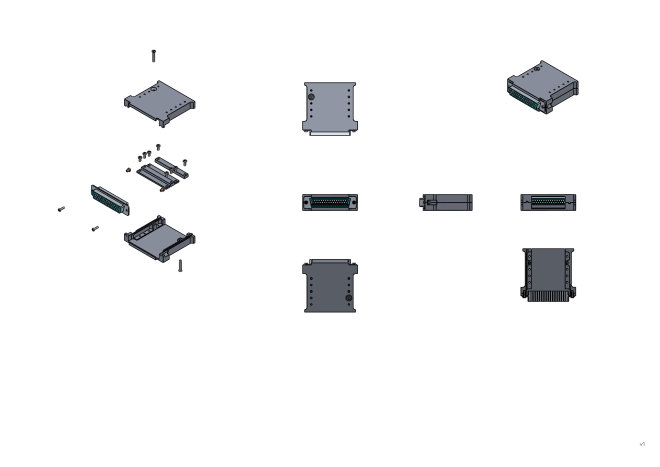
\includegraphics[width=0.75\columnwidth]{graphics/50-db50-housing.png}
  \caption{In-vacuum DB50 housing for octopus cable.}
  \label{fig:db50-housing}
\end{figure}
\chapter{Control of the Sagnac Speedmeter interferometer}
\label{c:speedmeter-control}

\note{Pillage paper}

    * Definition of degrees of freedom, powers, sidebands, etc...
    * Control loop design / noise budget
      * Inclusion of other noises, like seismic, thermal, electronic, etc. Calculation of noise budget.
      * Suspension hierarchical gain (handling ESD / coil ranges) (see labbook posts)
        * Crossover at ~200 Hz, show calculation of how high a frequency we need to control the arms to keep the power in there (see labbook)
      * Photodetector transimpedance
        * Set transimpedance so that signals are ~1 V...?
      * Mixing displacement and velocity signals
      * CDS overall gain setting
        * Set overall gain to not max the actuators on the suspensions, and provide ~1 V on the input to CDS
      * Whitening/dewhitening design (see labbook posts)
        * ADC input noise and effective number of bits (see labbook, Borja's email from 2015-08-28)
        * Set input voltage to CDS to be ~1/10th range, i.e. 1 V.
        * Make sure input noise from ADCs is 1/10th below the signal at all frequencies
    * Dark noise measurements of op-amp over long timescales (explain additional low frequency noise)
    * Note in ``outlook'' section on how we might verify how effective the optimal filter is compared to naive addition or a ``bad'' filter. Perhaps make a TF from an open port? Choose an optimally bad filter?
\chapter{Demonstration of a Plate Capacitor Electrostatic Drive Actuator}
\label{c:esd-concept}

* Introduce Holger's paper~\cite{Wittel2015} \etal{}, discuss need for high voltages
* Actuators usually couple noise, which is why magnets are usually on a stage above the test masses. This necessarily limits range, as any actuation performed by the magnets will be filtered by 1/f
* HV power supply design considerations (bleed resistor, voltage requirements, etc.)
* HV power supply current limiting circuit explanation (called ``foldback limiting'', see Horowitz and Hill p694)
* HV power supply heatsink considerations: power produced by MOSFETs at maximum current rating (100 mA, produces 25 W of heat - see datasheets) - chose heatsinks to dissipate this heat and make installation of the board easy (can screw TO-220 casing to L-shaped brackets)
* HV amplifier design: pressure and temperature cut-offs (explanation of how it works), input/output signals, choice of connectors, routing of signals for ease of assembly (front panel disconnect, etc.)
* Protective earthing (how the removal of the ground supply from the GEO supply will clamp ground to Earth beyond 18 V)
* HV amplifier transfer function, usign both HV output (via voltage divider) and monitor output
* HV amplifier monitor noise measurement
* This experiment will inform the main SSM experiment.
* 10 ohm resistor on output of amplifier design to damp resonant RCL modes: resistor adds loss, so lowers the Q associated with any suspension or cable pickups

* Discuss how Andreas' design (with my modifications) was a first prototype, and we decided to redesign it afterwards because of various problems: requirement for a 5V offset at all times, the heat production (due to quiescent current) of the PA98s, lack of switchable whitening. New design incorporates this stuff, along with significant digital signalling thought, and quad channels. New connector to the vacuum feedthrough, too.
* Discuss digital signalling design: avoiding ground loops, the DB25-37 converter board, pull-up resistors, etc. Mention that we considered EtherCAT for this but decided it was too expensive (needs a dedicated block inside the amplifier box)

As described in Chapter\,\ref{c:speedmeter-control}, the \ESD{} is best employed as a high frequency actuator...

\section{High voltage power supply}

\note{Describe indicator LEDs: their brightness is proportional to current, so while they are still lit the experiment is live.}

% ESD force gradient, from esd-ansys.pdf figure
\newcommand{\ESDFORCEGRAD}{\SI{-3.68}{\nano\newton\per\volt}}

% ESD maximum voltage
\newcommand{\ESDMAXVOLTAGE}{\SI{750}{\volt}}

% ESD maximum force, read from esd-ansys.pdf figure (gradient * voltage doesn't work because there's a non-zero y-intercept)
\newcommand{\ESDMAXFORCE}{\SI{-1.48e-6}{\micro\newton}}

There are a number of requirements for the plate capacitor's power supply. Due to the nature of the load--a capacitor formed from parallel plates--the power supply does not need to drive a significant current. On the other hand, the power supply will be modulated by the amplifier and sent to the plates, and the plates will actuate directly upon the test masses, and so any noise present upon the power supply output can potentially limit the sensitivity of the experiment. In order to achieve significant actuation, it is also necessary to provide a high voltage supply to the amplifier. Simulations conducted in the development of this experiment by group colleagues with the finite element modelling package \emph{ANSYS} have found that, for a mirror geometry resembling that of the \SSMEXPT{}'s ETMs, the force gradient will be \ESDFORCEGRAD{}, as shown in Figure\,\ref{fig:esd-ansys}. For a sufficient level of force actuation within the voltage isolation limit of our vacuum tank feedthroughs, a maximum feasible voltage across the capacitor appears to be in the region of \ESDMAXVOLTAGE{}, leading to a maximum mirror actuation force of \ESDMAXFORCE{}.
% ESD volts -> force from https://arran.physics.gla.ac.uk/wp/speedmeter/?p=4507

As this experiment is somewhat a technology demonstration for the main \SSMEXPT{}, it is worth keeping in mind its goals. For this reason, the power supply should provide suitably low output noise and sufficient channels for the purposes of the control of the full experiment.

\begin{figure}
  \centering
  \includegraphics[width=\columnwidth]{graphics/generated/from-python/70-esd-ansys.pdf}
  \caption{Simulations of the actuation force produced by the proposed ESD design upon a \SI{100}{\gram} cylindrical test mass of diameter \SI{48.6}{\milli\meter} and depth \SI{24.5}{\milli\meter} resembling that of the \SSM experiment's ETMs. The plate separation and the position of the mirror with respect to the plates influence the level of force produced. \checkme{In practice it is most beneficial to have the mirror centre of mass aligned to the edge of the plates and the plates as close as possible to the mirror without touching.}}
  \label{fig:esd-ansys}
\end{figure}

\section{High voltage amplifier}

A means of controlling the \AC{} component of the high voltage (\gls{HV}) supply is necessary to perform frequency-dependent corrections upon the mirror. Although the ESD, and indeed the \SSM{} experiment, primarily require corrections at lower frequencies where seismic noise is dominant, it is beneficial to utilise an amplifier which can provide actuation up to many tens, if not hundreds, of \SI{}{\kilo\hertz}. This is to provide a transfer function which is flat across the vast majority of each experiment's measurement band, avoiding the roll-off at high frequencies due to the integrated circuits utilised within the high voltage amplifier. A flat transfer function makes the calibration of the actuator plant as simple as possible. Another benefit of having a high bandwidth amplifier is the possibility to use it for common mode control loops, where laser frequency stabilisation can be split between feedback to the laser's piezoelectric transducer and actuators on the test masses.

The key component of a high bandwidth amplifier is the power op-amp. This class of op-amps typically utilises a \MOSFET{} design, and can provide high voltage output given a low voltage input. As an example, the Apex PA95 op-amps used in Advanced LIGO's \ESDs{} provide up to \SI{900}{\volt} output up to a frequency of around \SI{15}{\kilo\hertz}, and up to \SI{50}{\volt} at \SI{250}{\kilo\hertz}. The PA98 op-amp, also from Apex, provides an output of \SI{450}{\volt} nominally up to \SI{60}{\kilo\hertz}, potentially up to \SI{500}{\kilo\hertz} for a low capacitive load. For the purposes of this experiment, the choice was made to use the PA98 op-amp to provide the ability to study the effect of the actuator across a very wide bandwidth. To this end, an amplifier circuit utilising the PA98 was built based on a design used for the \AEIPROTOTYPE{}. Two notable modifications have been made, both of which are safety enhancements.

% claim about voltage output of PA95 comes from figure ``Power Response'' on p3 of PA95 datasheet (https://www.apexanalog.com/resources/products/pa95u.pdf)
% claim about voltage output of PA98 comes from figure 8: ``power Response'' on p7 of PA98 datasheet (https://www.apexanalog.com/resources/products/pa98u.pdf)

The first modification is the use of alternative high voltage connectors. The \AEIPROTOTYPE{} design called for two \emph{SHV} connectors carrying the separate +\gls{HV} and -\gls{HV} rails to the vacuum feedthrough on separate cables, with the vacuum system acting as the virtual ground between the two rails. While both cables are connected, this system is safe; however, if one cable is disconnected, a fault with the amplifier circuit can cause the vacuum system to become live. To avoid the possibility of this situation ocurring in the \SSM{}, a Bulgin-type connector was used to combine the +\gls{HV} and -\gls{HV} rails in a single connector and cable. With this style of connector it is not possible to disconnect from the vacuum system any single \gls{HV} rail while leaving the other connected.

The second modification made to the amplifier circuit was the addition of a safety interlock mechanism. The breakdown voltage of the plate capacitors as a function of pressure, given by Paschen's Law, has a minimum in the region of \SI{e3}{} to \SI{e7}{\milli\bar} depending on the separation of the anode and cathode. In addition, related effects such as surface tracking can lead to arcing at voltages above \SI{50}{\volt} in low vacuum. Although the use of high voltage plate capacitors is in general safe at both atmospheric pressure and high vacuum (below \SI{e-6}{\milli\bar}), the act of pumping gas out of the vacuum system necessarily passes through pressures at which arcing can occur, and so a safety mechanism was decided to be necessary.

To prevent the possibility of arcing, a cut-off function was added to the circuit to prevent high voltage output unless a voltage above \SI{5}{\volt} is applied across terminals on the enclosure. This threshold was chosen based on the monitor output voltage provided by a pressure gauge attached to the vacuum system. This varies logarithmically from \SI{0}{} to \SI{10}{\volt} for pressures between standard atmosphere and ultra-high vacuum. A voltage above \SI{5}{\volt} indicates a pressure below \SI{e-5}{\milli\bar}.

% pressure vs voltage claim from speedmeter labbook, at https://arran.physics.gla.ac.uk/wp/speedmeter/2015/01/30/esd-hv-amplifier-pressure-cutoff/

\begin{figure}
  \centering
  \includegraphics[width=\columnwidth]{graphics/generated/from-python/70-esd-paschen.pdf}
  \caption{The minimum breakdown voltage between the two plates of the \ESD{} for different separations. This is calculated using Paschen's Law, assuming nitrogen gas and a flat plate geometry. The effect is a lot more complicated for real systems, where different plate geometries will have different relationships, but the steep slope at lower pressures shown here indicates that the apparatus used in the \ESD{} experiment will very likely avoid any problems with arcing as long as a suitable pressure-based interlock is utilised in the design of the electronics.}
  \label{fig:esd-paschen}
\end{figure}

\subsection{Description of signal and noise paths}
The \gls{HV} amplifier is designed to have a very wide bandwidth, and the power amplifier has been chosen with this goal in mind. The amplifier circuit, however, contains more than just the power amplifier, but also filtering and safety mechanisms in the form of additional integrated circuits and other passive and active components. The control input from \gls{CDS} is a differential signal, and any common mode noise that may have entered in each channel on the way to the amplifier is to a great extent removed by a balanced line receiver present at the amplifier's input. This outputs a single-ended signal which which is split into two parts, with one being inverted via a buffer op-amp, and these two signals are sent to their respective power amplifiers. Additional op-amps also control the supply voltage provided to each power amplifier. To prevent high current in-rush when the power supply is attached to the amplifier--as reactive components such as capacitors and inductors charge--an op-amp limits the current to a level low enough for the power supply to provide without locking.

In \gls{CDS}, the signal $S$ is sent from the digital to the analogue domain via \gls{ADC}s, where it is split into two channels, $A$ and $B$, containing the same signal but with opposite sign. These signals are sent to the amplifier in a two-core cable. As laboratories inevitably contain stray electromagnetic fields, channels $A$ and $B$ pick up noise $n_{A}$ and $n_{B}$, respectively:
\begin{align}
  A &= S + n_{A}, \\
  B &= -S + n_{B}.
\end{align}
These noise sources can be further represented in terms of common and differential modes at the amplifier input, $n_{\left(+\right)}$ and $n_{\left(-\right)}$, respectively:
\begin{align}
  n_{\left(+\right)} &= n_{A} + n_{B}, \\
  n_{\left(-\right)} &= n_{A} - n_{B}.
\end{align}
The purpose of this so-called \emph{differential sending} is to allow $n_{\left(+\right)}$ to be cancelled at the amplifier. Injecting channels $A$ and $B$ into an op-amp with high \emph{common-mode rejection}, we get:
\begin{align}
  S_{\text{out}} &= G_{\left(-\right)} \left(A - B\right) + G_{\left(+\right)} \frac{\left(A + B\right)}{2} \\
                 &= G_{\left(-\right)} \left(2S + n_{\left(-\right)}\right) + G_{\left(+\right)} \frac{n_{\left(+\right)}}{2},
\end{align}
where $G_{\left(-\right)}$ and $G_{\left(+\right)}$ are the op-amp's differential and common mode (power) gains, respectively.

As the original signal produced by \gls{CDS} is inverted in one channel, each channel contains purely differential signal, but the noise picked up by each channel is in both the differential and common modes. An op-amp's ability to remove common mode noise between its inputs is typically expressed as its \emph{common mode rejection ratio} (\gls{CMRR}), defined as the logarithm of the ratio of the differential and common mode gains:
\begin{equation}
  \text{CMRR} = 20 \log_{10} \left( \frac{G_{\left(-\right)}}{G_{\left(+\right)}} \right),
\end{equation}
with the resulting number expressed in decibels. Within the amplifier, the signals are subtracted by an AD829 with $\text{CMRR} = 120$ (at \SI{1}{\kilo\hertz}) configured with $G_{\left(-\right)} = 1$, resulting in only $5 \times 10^{-7} n_{\left(+\right)}$ making its way to the output (neglecting imbalances in nearby components such as resistors), making it comparible or less significant than the output noise of the op-amp itself. As the channels are physically close to one another as they are sent to the amplifier--contained within the same shielded cable--$n_{\left(-\right)}$ also tends to be small for frequencies below a few hundred \SI{}{\giga\hertz}, or less than \SI{}{\milli\meter} wavelength. Using a receiving op-amp with sufficiently high \gls{CMRR}, a desired control signal can be sent from \gls{CDS} to the amplifier without the addition of significant noise.

% small differential noise claim: f = c/lambda, assume lambda has to be less than the channel separation in a cable, roughly 1mm, so 3e8 / 1e-3 = 3e11 = 300 GHz.

The gain of the amplifier can be determined from inspection of the path an input signal takes to the output... \note{discuss how gain arises in circuit}

\subsection{Transfer functions}
\note{Describe measurement: use of voltage divider, need to take into account impedance of the send box in its design, bandwidth of each measurement: CDS up to 10 kHz, SR785 up to 100 kHz, Agilent up to MHz. Describe monitor and \gls{HV} rail outputs, and how we avoid ground loops (isolated case from double LEMO and monitor outputs.}

The presence of stray capacitance at the inputs and outputs of these additional integrated circuits can have an influence upon the overall response of the amplifier as a function of frequency. It is beneficial, therefore, to check that the frequency response of the amplifier is dominated by the power amplifier and not by some auxiliary component.

\subsection{Noise measurements}

\note{Spectral density noise with SR785}

\section{The Experiment}

\subsection{Transfer functions}
\note{Hopefully these are flat, just like the actuator TFs, once the cavity effect is removed...}

\section{Outlook}
\chapter{Integration of Slow Control Channels in LIGO CDS}
\label{c:slow-controls-integration}

% appendices
\appendix
\chapter{\label{a:simulation-tools}Simulation Tools}
How to build simulations in both tools...

\note{Mention about difference in homodyne angles between Optickle and Finesse - empirical formula on speedmeter labbook post from end of 2015/early 2016}

\section{Finesse}

\section{Optickle}
Optickle is a tool primarily designed to produce a series of matrices as outputs. As it is based in \MATLAB, it is possible to study the behaviour of the code to determine its capabilities and limitations. This section attempts to explain the basic operation of the primary feature that Optickle provides: the \lstinline{tickle} function.

In order to simulate an interferometer, an optical environment is created into which optics, sensors and links between optics may be defined. The primary output of Optickle is a transfer matrix mapping \emph{drives} of each optic in the system to probes within that system. A drive is simply a degree of freedom of an optic, such as longitudinal motion of a mirror. Probes are the simulation equivalent of photodetectors, but can be lossless and can perform arbitrary RF demodulations. Another useful output is the quantum noise spectral density at a probe. Dividing the noise spectral density at a probe by a suitable linear combination of optical transfer functions--a degree of freedom of the interferometer---results in the probe's noise-to-signal ratio, or sensitivity, to that degree of freedom.

Whilst Optickle's code is extensive, the vast majority can be categorised into a few sets of routines:

\begin{itemize}
  \item defining parameters and matrices for various types of optic, including the field, reaction and noise transfer matrices;
  \item defining manipulations of sets of matrices to produce transfer functions and noise spectral densities for optics and sensors within the system.
\end{itemize}

Once an optical system has been defined by the user, a call to the \lstinline{tickle} function results in a number of operations being performed:
\begin{itemize}
  \item the construction of matrices mapping the drives of an optic to the fields in the interferometer, and each field to each other field;
  \item the constructi
\end{itemize}

\subsection{Drive and Field Maps}
The drive-to-field matrix produced by \lstinline{tickle} is the mapping between a \emph{drive} of an optic---a degree of freedom such as longitudinal motion of a mirror---to the corresponding fields in the interferometer. A \emph{field} is in this case the amplitude of the light between a particular pair of optics or sensors for a given wavelength. The individual transfer functions are themselves products of each optic's drive matrix (which converts a force input at the test mass to a phase change in the reflected and transmitted light, via the optic's mechanical transfer function) and a phase matrix defining the phase change light would have travelling between each optic in the system. The field-to-drive matrix is also produced in a similar way, but this time maps the interaction that light fields have with the optical drives--i.e. the effect of radiation pressure.

The field-to-field matrix is a similar mapping to the drive-to-field matrix, but this instead maps each field to each other field. As such, with this matrix the propagation of input light from lasers or vacuum injection to an arbitrary part of the interferometer can be calculated, albeit without the effect of radiation pressure.

The effect of field amplitudes propagating to other fields, optics modifying incident fields, and fields modifying optics can be collected together into a \emph{propagation matrix} $\mathbf{M}_{\text{AC}}$.

\subsection{Calculation of Field Amplitudes}
The field amplitudes within the interferometer $\vec{v}_{\text{AC}}$ can be determined by calculating the steady-state solution of the optical system to a given excitation. An excitation is, for instance, the injection of light. The field amplitudes within the interferometer are of course determined by the excitation of the interferometer by external light injection, but in general they are also influenced by the signal sidebands produced by the modulation of optics within the interferometer at non-zero frequencies. Furthermore, the presence of optics will alter the injected excitation. The field amplitudes within the interferometer therefore depend not only on the excitation but also on the existing field amplitudes, analogous to feedback systems. In the initial state these fields are zero and so the interferometer's field amplitude vector is simply equal to the excitation vector, i.e. $\vec{v}_{\text{AC}} = \vec{v}_{\text{exc}}$. The stored light will increase until eventually the injected excitation is equal to the light power lost in the interferometer. Once this condition is reached the interferometer is in its steady-state.

The steady state condition can be solved numerically using matrix inversion. As described above, the field amplitudes depend not only on the input but also on the field amplitudes themselves, i.e.
\begin{equation}
  \vec{v}_{\text{AC}} = \mathbf{M}_{\text{AC}} \vec{v}_{\text{AC}} + \vec{v}_{\text{exc}},
\end{equation}
where $\mathbf{M}_{\text{AC}}$ is the phase matrix specified earlier. This equation can be solved as such:
\begin{equation}
  \vec{v}_{\text{AC}} = \frac{\vec{v}_{\text{exc}}}{1 - \mathbf{M}_{\text{AC}}}.
\end{equation}
Since $\mathbf{M}_{\text{AC}}$ is a matrix and $\vec{v}_{\text{AC}}$ and $\vec{v}_{\text{exc}}$ are vectors, the problem can be represented as the matrix equation:
\begin{equation}
  \vec{v}_{\text{AC}} = \left( \mathbb{I} - \mathbf{M}_{\text{AC}} \right)^{-1} \vec{v}_{\text{exc}},
\end{equation}
where $\mathbb{I}$ is the identity matrix. The calculation of the field amplitudes in the interferometer therefore becomes a task of finding the inverse of $\mathbb{I} - \mathbf{M}_{\text{AC}}$.

\subsection{Probe Signals}
With the steady-state field amplitudes, the signals produced by the interferometer can be determined with the application of a \emph{probe matrix} $\mathbf{M}_{\text{probe}}$ which maps the fields in the interferometer to probes contained within the interferometer. Since the fields amplitudes are determined for every wavelength under consideration, it is possible to calculate the signals that would appear on photodetector circuits implementing RF demodulation. The probe matrix contains complex amplitudes to transform the fields at the location of the probe by the required amount given the demodulation frequencies and phase angles. The probe signals are therefore defined as:
\begin{equation}
  \vec{v}_{\text{probe}} = \mathbf{M}_{\text{probe}} \left( \mathbb{I} - \mathbf{M}_{\text{AC}} \right)^{-1} \vec{v}_{\text{exc}}.
\end{equation}

\subsection{Calculation of Transfer Functions}
The operation of calculating the probe signals from the field amplitudes in the interferometer can be repeated for arbitrary frequencies of excitation to produce a three-dimensional drive-to-probe transfer matrix. This represents the transfer function from each optic's degree of freedom to each probe. As such, the signal from a particular \emph{interferometer} degree of freedom can be constructed via a linear combination of optic degrees of freedom transfer functions. The differential arm degree of freedom transfer function for a \MI to its asymmetric port, for instance, can be calculated by extracting the transfer function of each end test mass to a probe situated at the asymmetric port and taking the difference of the two \note{, as shown in Equation x in Section y.}

\subsection{Probe Quantum Noise}
...

\section{Reflection Phase Convention}
\label{a:reflection-phase}
\note{Difference between Optickle and Finesse sign conventions for transmission and reflection. See footnote 1 on p2 of T1100110 for more details.}

\chapter{\label{a:alignment-control}Alignment Control}
As shown throughout this thesis, the use of optical cavities can greatly enhance interferometric length measurement techniques. \note{Whilst} the initial alignment of most ``simple'' Michelson interferometers is relatively straightforward, the inclusion of optical cavities to the arms of the Michelson, and indeed other interferometer topologies, provides an additional challenge in obtaining and maintaining lock, both in the angular and longitudinal degrees of freedom.

Recent interferometric experiments in the \GLASGOWTENM have required a high degree of sensitivity and thus high finesse optical cavities \note{(cite Neil's thesis, paper)}. Test masses, suspended from multiple pendulum stages, are constrained in angular and longitudinal degrees of freedom by voice coil and magnet pairs (see, for example, \note{Figure X from Waveguide chapter}). As initial alignment of optics is a task undertaken infrequently, and not part of any closed control loop, it is safe to use actuators on stages above the test mass. This has two advantages:
\begin{itemize}
 \item the main control loops to produce fast corrections to the test mass positions during data acquisition need not share the same actuators as the initial alignment;
 \item and the dc alignment signal is filtered by the pendulum system so as not to contaminate the (typically audio frequency) measurement band.
\end{itemize}
As the task of alignment is an open loop system, it is not an efficient use of resources to dedicate high dynamic range ADC channels. It is therefore beneficial to develop a system for initial alignment using separate control software and hardware to the main system.

\section{Requirements}
Given the experience of lab colleagues from previous experiments, the requirements of such an alignment control system boil down to the following:
\begin{itemize}
 \item ability to align a given optic across the face of its neighbours;
 \item ability to control the alignment of all suspensions from a central location;
 \item relatively low cost compared to full dynamic range experimental ADC channels.
\end{itemize}
From previous experience with other control systems, it is also desirable to have the following features:
\begin{itemize}
 \item reproduceability of prior states;
 \item ability to control suspension alignment from any location.
\end{itemize}
Previous experience with commercial control equipment has led to some issues. Commercial hardware is typically at the mercy of proprietary software from the same vendor sometimes designed as an afterthought. Once a line of lab equipment is no longer popular it is also at the discretion of the manufacturer to maintain and support the equipment still in use. Due to these issues, along with the lists of requirements above, the seemingly obvious solution pointed towards the use of a distributed, networked system of individual suspension controllers using open hardware and software.

\section{Open Hardware and Software}
In recent years there has been a trend towards the production of low cost, open hardware. One such line of devices is the \emph{Arduino}, with hobby-level units available to the general public with open programmable interfaces, and a vibrant community of volunteers offering support.

% end
\backmatter

% bibliography
\addcontentsline{toc}{chapter}{Bibliography}
\printbibliography

\end{document}